\chapter{Sistema de ejecución de trayectorias}
\label{cap: trayectorias}

En este capítulo se aborda la construcción de un sistema de cálculo y ejecución automática de movimientos para el robot colaborativo UR. El sistema utiliza como soporte software la interfaz proporcionada por ROS2 Humble y el controlador Moveit. 

El capítulo empieza haciendo una breve descripción del problema mientras resalta la importancia de los tres pilares fundamentales en los que debe sustentarse el sistema: el entorno virtual, el sistema de cálculo y ejecución de trayectorias y el control de velocidad. A continuación se procede a describir la metodología seguida en el desarrollo de cada uno de estos paquetes. Finalmente se pasa a la sección de resultados, donde se mostrará una validación para cada bloque y se comentarán las limitaciones del sistema implementado, así como sus mayores ventajas.

El código descrito en este capítulo se encuentra disponible en el repositorio GitHub del proyecto \cite{repo_github_TFM_MiguelLerinAlonso}. Los nodos de ROS2 que representan dichas tareas pertenecen al paquete \textit{trayectories}\footnote{Disponible en el direccionamiento: \textit{./workspace/ros\_ur\_driver/src/trayectories}}

\section{Introducción al problema}
El movimiento efectuado por manipulador robótico se basa en los fundamentos del cálculo de la cinemáticas directa e inversa. Actualmente se dispone del aparato matemático suficiente para definir la posición adoptada por el manipulador robótico a través de su configuración articular o el punto del espacio en el que se ubica el \acrshort{TCP}.

Sin embargo, el empleo de robots industriales en estaciones de fabricación ha de tomar en cuenta no únicamente el espacio de movimiento del robot en su totalidad, si no que también ha de introducir restricciones en aspectos como:
\begin{itemize}
    \item La presencia de objetos físicos con los que puede colisionar.
    \item El uso de herramientas acopladas a su \acrshort{TCP}.
    \item La definición de un sistema de cálculo que minimice movimientos y consumo energético.
    \item Control de parámetros de ejecución como la velocidad o las inercias asociadas a cada eslabón.
    \item Posiciones del manipulador que impliquen un mal funcionamiento al final
\end{itemize}

Los entornos de trabajo software como ROS2 facilitan el cálculo de dichos aspectos y proporcionan al usuario una interfaz en la que dispone de total libertad para imponer las restricciones que crea convenientes en la tarea de cálculo y ejecución de movimientos robóticos. Dependiendo del modelo de cálculo empleado para resolver las ecuaciones de la cinemática, es posible ponderar dichas restricciones. Esto es, se puede priorizar evitar la colisión contra elementos externos frente a la minimización de recorrido o establecer la velocidad de ejecución como un cálculo separado.

La mayor dificultad que conlleva el empleo de este tipo de sistemas es la definición de un algoritmo de cálculo que tenga en cuenta todas estas restricciones y además pueda efectuar movimientos con cierta complejidad (como es en el caso de este trabajo con el resultado del slicer no planar). Desde la primera versión de \acrshort{ROS} y ROS2 han surgido multitud de algoritmos de cálculo de trayectorias a partir de la cinemática inversa, como son el caso de Moveit\cite{moveit_documentacion}, TrackIK\cite{tracik}, KDL\cite{kdl}, Ruckig\cite{ruckig} o Tesseract\cite{tesseract} entre otros. Sin embargo, en muchas ocasiones se desconoce si la capacidad de este tipo de algoritmos es suficiente para procesar y efectuar trayectorias complejas en espacios reducidos. 

Por estos motivos el desarrollo de un sistema automático de ejecución de trayectorias debe pasar por tres fases diferenciadas: una primera en la que se define el entorno de trabajo robótico real en el modelo implementado con ROS2, una segunda en la que se evalúa las capacidad del algoritmo utilizado para el trazado de trayectorias complejas y una tercera en la que se valida la integración de diferentes sistemas de control -como por ejemplo es el control de la velocidad de ejecución- sobre el trazado calculado.

\section{Metodología}

En las siguientes líneas se describe el procedimiento seguido en cada una de las etapas descritas anteriormente. Se comienza presentando las principales herramientas empleadas para posteriormente indicar el uso que se les ha dado y las valoraciones realizadas para escoger una alternativa sobre el resto.

\subsection{Construcción del entorno virtual}
El modelo virtual del robot se construye utilizando tres herramientas de software fundamentales: la interfaz proporcionada por ROS2 Humble para la creación y gestión de mensajes entre el robot y la computadora central; el controlador MoveIt para el cálculo y planificación de trayectorias en el espacio; el controlador de UR, que proporciona una capa de software intermedia para el modelado y control de sus robots; y la interfaz gráfica proporcionada por RViz para el manejo del robot en el entorno real y simulado.

La capa de control intermedia proporcionada por el controlador de UR sirve como plantilla de invocación y lanzamiento de varios equipos de la compañía, facilitando la gestión de diferentes mensajes y el procedimiento de cálculo y ejecución de movimientos. La documentación oficial indica que este controlador se encuentra especialmente optimizado para el sistema de planificación y ejecución de trayectorias MoveIt, el cual ha servido de referencia durante su etapa de diseño. Por este motivo se escoge a MoveIt como principal software de cálculo y gestión de movimientos, en concreto a su versión optimizada para ROS2 Humble que es la que se utiliza en este proyecto. El visor RViz se escoge como interfaz gráfica de referencia por su capacidad para integrarse rápidamente con las trayectorias planificadas por MoveIt.

\subsubsection*{Modelo virtual del robot}
\hypertarget{Modelo virtual del robot}{}
\bookmark[level=subsubsection,dest=Modelo virtual del robot]{Modelo virtual del robot}
\label{sec: modelo virtual del robot}

Después de instalar cada uno de los elementos en el computador central siguiendo sus respectivas instrucciones, se procede a insertar un modelo de robot UR con ayuda del controlador UR. Este controlador basa su funcionamiento en cuatro paquetes especializados en las siguientes tareas:
\begin{itemize}
    \item Extraer e integrar la calibración del robot UR real
    \item Implementar los controladores específicos para el movimiento del robot
    \item Definir la capa intermedia de mensajes entre el robot UR y el computador central
    \item Configurar automáticamente las herramientas hardware y software necesarias para el movimiento del manipulador utilizando ROS2
\end{itemize}

Además de estos paquetes, el controlador pone a disposición del usuario ejemplos de configuración de varios modelos de la compañía. De modo que el único requisito sea la definición de la unidad empleada a través de un archivo \acrshort{YAML} que especifique su calibración, la IP del robot en el entorno de programación real y los programas de gestión de hardware empleados. Estos ejemplos se definen en un tipo de archivo de python compatible con ROS2 conocidos como archivos de lanzamiento o archivos \textit{launch}.

El controlador asume la gestión del modelo a través de dos paquetes software de ROS2 complementarios: la descripción del robot y su entorno de trabajo virtualizado y la gestión de mensajes, sensores y actuadores \footnote{Ambos paquetes se encuentran instalados en la ruta \textit{$./workspace/ros\_ur\_driver/src$}}. La tarea del ingeniero de este modo pasa a la definición de los límites de la cinemática del robot modificando únicamente los valores presentes en archivos \acrshort{YAML} especializados, ya que será el controlador de UR y MoveIt los responsables de generar automáticamente los archivos de retrocompatibles para el modelo de ROS2.

La Figura \ref{fig: archivos modelo virtual UR} muestra capturas de pantalla de parte de los archivos implicados en la descripción del modelo virtual del UR. Estos archivos de descripción del robot son:

\begin{itemize}
    \item \textbf{default\_kinematics}: Para definir la posición y orientación predeterminadas de cada articulación del UR virtualizado.
    \item \textbf{joint\_limits:} Para especificar los limites de posición, velocidad y esfuerzo articular que debe implementar el modelo de cálculo cinemático.
    \item \textbf{physical\_parameters:} Para establecer las desviaciones reales entre cada eslabón y articulación del robot real respecto del virtualizado en cuando a los modelos base utilizados para la cinemática y la dinámica. Estos valores se pueden introducir manualmente disponiendo de la calibración de la unidad empleada o automáticamente recurriendo al sistema de extracción de calibración del controlador UR.
    \item \textbf{visual\_parameters:} Para representar el modelo tridimensional del manipulador en la interfaz gráfica de RViz y efectuar las animaciones correspondientes al cálculo de MoveIt.
\end{itemize} 

\begin{figure}[h!]
    \centering
    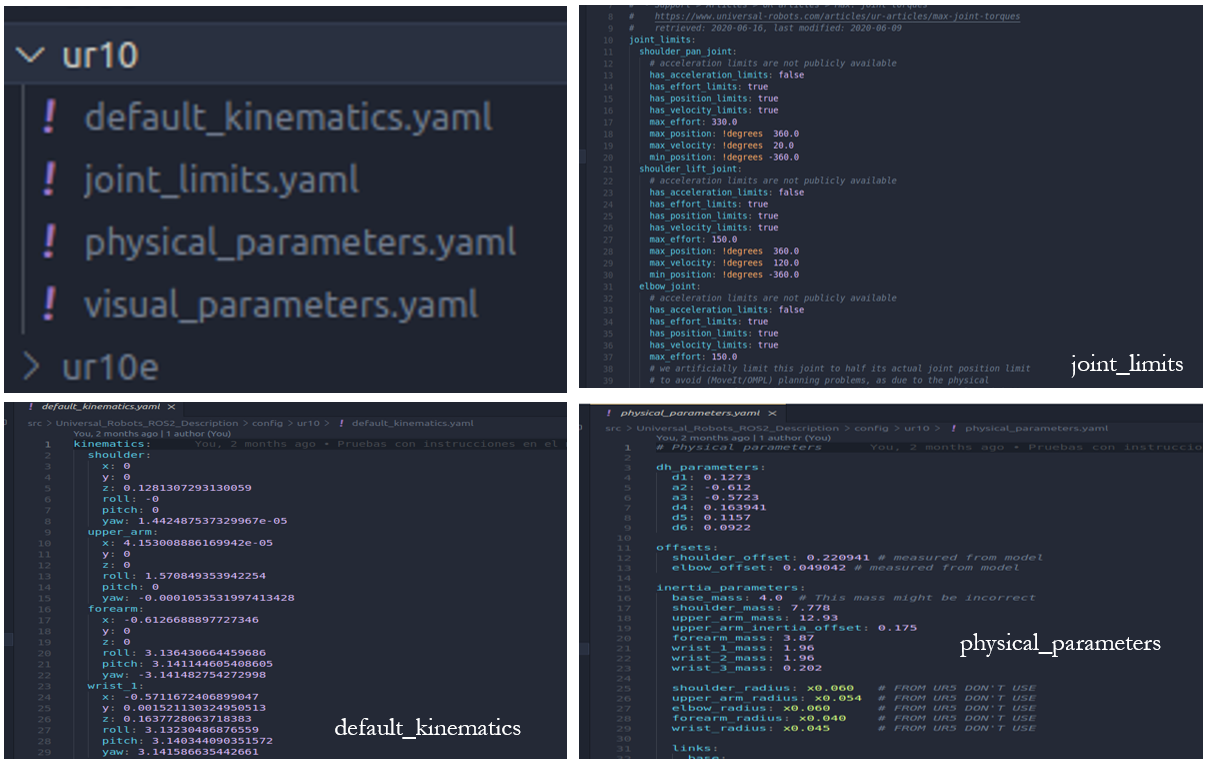
\includegraphics[scale=0.5]{figuras/archivos_modelo_virtual_UR.png}
    \caption{Archivos de definición de modelo virtual del UR}
    \label{fig: archivos modelo virtual UR}
\end{figure}

\subsubsection*{Entorno de trabajo}
\hypertarget{Entorno de trabajo trayectorias}{}
\bookmark[level=subsubsection,dest=Entorno de trabajo trayectorias]{Entorno de trabajo}

El siguiente paso es la definición de un entorno de trabajo virtual para el movimiento del robot. Esto es, disponer de un conjunto de elementos definidos a través de un modelo tridimensional que impongan restricciones en el espacio de movimiento del robot. 

La integración de este tipo de elementos se utiliza para que el algoritmo de cálculo pueda redefinir el espació útil de trabajo para el robot y se eviten colisiones, gestione la posibilidad de adoptar poses que comprometan su integridad física o trace trayectos intermedios seguros entre la trayectoria comandada y el punto actual en el que se ubica el \acrshort{TCP} del manipulador.

Tanto ROS2 como MoveIt permiten la definición de elementos en el entorno virtual a través de modelos tridimensionales definidos como archivos \acrshort{STL}. La construcción del entorno de trabajo se basa en la implementación de un archivo de xacro en el que se enlazan los distintos elementos de la estación al modelo virtualizado del robot. 

Es decir, se construye una cadena cinemática mayor a partir de elementos de menor nivel de abstracción como son los eslabones del robot, el modelo de la mesa de trabajo, la plataforma de impresión o el soporte para el sensor láser y el extrusor. Se utiliza como origen de coordenadas de referencia la base del robot, de forma que el resto de elementos -tanto eslabones robóticos como herramientas- se enlazan a él indicando el elemento previo de la cadena cinemática y la posición-orientación relativa al mismo. 

Las siguientes figuras muestran ejemplos del código empleado en la xacro para enlazar el modelo tridimensional de la cama de impresión y la mesa de trabajo. Nótese cómo los campos de mayor importancia son aquellos que indican (1) el nombre del elemento virtualizado, (2) la ruta donde encontrar el modelo \acrshort{CAD}, (3) el factor de escala y (4) la posición y orientación del centro de inercia respecto al elemento anterior de la cadena cinemática. 

\begin{figure}[h!]
    \centering
    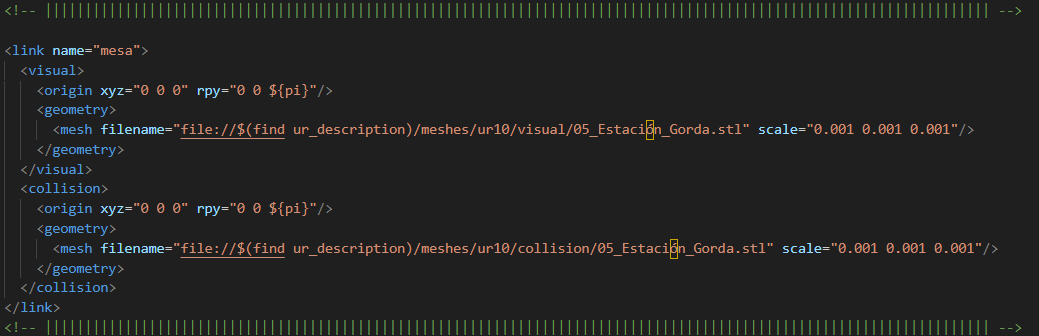
\includegraphics[scale=0.50]{figuras/posicionamiento xacro mesa estacion.png}
    \caption{Xacro posicionamiento de mesa}
    \label{fig: posicionamiento xacro mesa estacion}
\end{figure}

\begin{figure}[h!]
    \centering
    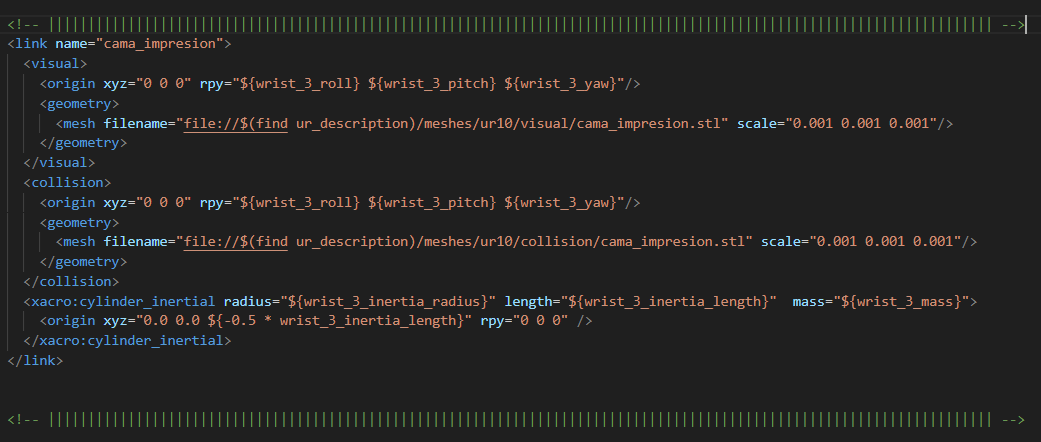
\includegraphics[scale=0.50]{figuras/posicionamiento xacro cama impresion.png}
    \caption{Xacro posicionamiento de cama de impresión}
    \label{fig: poscionamiento xacro cama impresión}
\end{figure}

En el caso de la mesa (Figura \ref{fig: posicionamiento xacro mesa estacion}) el elemento previo es la articulación base  del modelo UR, por lo que considerarse sistema de referencia principal se utiliza una inserción de coordenadas directas. En el caso de la cama de impresión (Figura \ref{fig: poscionamiento xacro cama impresión}), al encontrarse acoplada a la muñeca número 3, se inserta el nombre del centro de inercia de dicho eslabón para indicar un posicionamiento relativo.

La Figura \ref{fig: entorno virtual robot mesa cama} muestra como resultado la interfaz combinada de RViz y MoveIt utilizada en este proyecto. En ella se muestra el entorno virtual definido en esta sección. La mesa de la estación y la cama de impresión se encuentran señaladas en color rojo indicando que son elementos externos unidos a la cadena cinemática principal, la del modelo robótico UR. De forma análoga a la Figura \ref{fig: estacion_NPAM_sin_estruxor} se ubica el manipulador robótico con la cama de impresión y el soporte para el sensor láser en la misma posición en la que se ubican en la estación real.

\begin{figure}[h!]
    \centering
    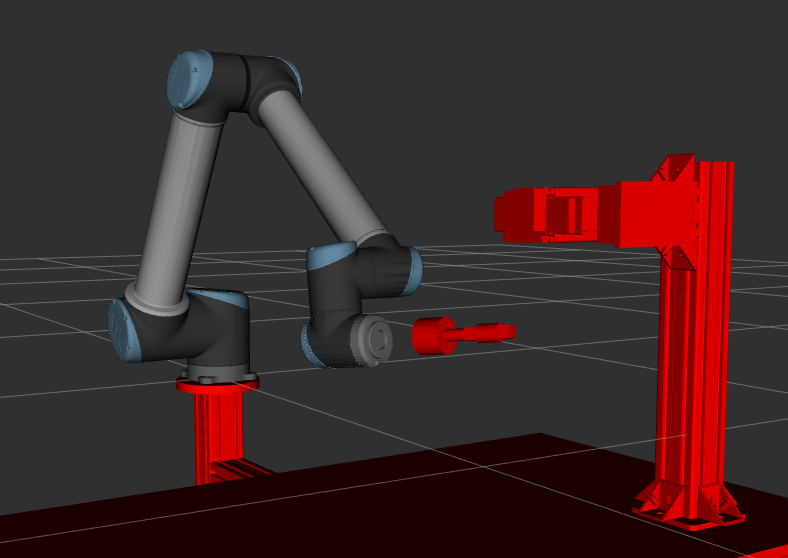
\includegraphics[scale=0.30]{figuras/entorno_virutal_cad_cama.png}
    \caption{Entorno virtual construido}
    \label{fig: entorno virtual robot mesa cama}
\end{figure}

El modelo \acrshort{CAD} de la cama de impresión se ubica como un elemento rígido flotante acoplado a la muñeca número 3 debido a la falta de un modelo tridimensional del sistema de acople rápido de herramientas del que dispone el cobot real. Para corregir esta problemática, se realizaron ajustes sucesivos a los parámetros de posición y orientación respecto a dicha articulación mediante un proceso en el que se tomaba el modelo \acrshort{CAD} de la cama de impresión y su calibración intrínseca.

\subsection{Movimiento del robot}

El cálculo de trayectorias suele ser tarea de un sistema informático programado especialmente para ello. En entorno software como ROS2, diseñados para la introducción de cualquier modelo de robot en ellos resulta especialmente útil el desarrollo de un modelo in situ para el manipulador si este ha sido diseñado desde etapas muy tempranas. No obstante, el uso de robots comerciales -independientemente de que se traten de modelos convencionales o colaborativos- necesita de un sistema de control y regulación de sus actuadores más preciso para evitar daños sobre la propia maquinaria y los operarios que la manejan.

Es decir, es común que los mayores fabricantes del mercado aporten un sistema de control automático de sus equipos. La mayoría de estos sistemas están pensados tomando como referencia ciertos controladores disponibles en la literatura de código abierto. Este es el caso del controlador de UR descrito en la sección \ref{sec: modelo virtual del robot} con el sistema de cálculo de trayectorias MoveIt. 

En las siguientes líneas se expone la implementación de dicho sistema para leer la matriz de puntos provenientes, calcular un conjunto de poses articulares que lleven al \acrshort{TCP} hacia dichos puntos y mandar la orden de ejecución de dichas posiciones al cobot.

\subsubsection*{Cálculo de trayectorias}
\hypertarget{Cálculo de trayectorias}{}
\bookmark[level=subsubsection,dest=Cálculo de trayectorias]{Cálculo de trayectorias}

El entorno virtual definido anteriormente sirve para imponer restricciones al movimiento del robot en su espacio de trabajo. En el caso de este proyecto, la restricción que se ha ponderado como más importante ha sido la supresión de colisiones con los elementos del entorno de trabajo. 

Dicha restricción está asociada a una solución de compromiso con la correspondiente a la minimización de distancia recorrida. Esto es, se prefiere que el robot efectúe movimientos largos y alejados de los elementos que suponen un riesgo de colisión antes de comprometer la integridad del resto de equipos de la estación.

La documentación oficial de la versión de MoveIt para ROS2 Humble \cite{moveit_documentacion} indica que el controlador es capaz de obtener la cinemática directa e inversa para una serie de puntos definidos respecto del sistema de coordenadas ubicado en la base del robot, que se toma como origen de coordenadas globales. 

El cálculo de las posiciones necesarias para cada elemento de la cadena cinemática definida para el entorno virtual se realiza automáticamente a través de los servicios de ROS2 \textit{GetPositionFK} y \textit{GetPositionIK}. Estos servicios tan sólo proporcionan un conjunto de puntos en el espacio cartesiano y de posiciones articulares respectivamente. En otras palabras, no se aporta ninguna información respecto al tiempo de ejecución de cada pose, la velocidad de movimiento o las restricciones aplicadas.

El servicio ROS2 responsable de obtener un mensaje que exprese el movimiento por realizar es conocido como \textit{GetCartesianPath}. Dicho es aportado por el controlador MoveIt e implementa un algoritmo que permite hallar distintas soluciones al movimiento robótico a través de la cinemática inversa. Dicho algoritmo no se encuentra accesible al público, por lo que únicamente se dispone de una interfaz en forma de mensajes ROS2.

La interfaz sirve para definir las restricciones que debe tener en cuenta el algoritmo en cuanto a espacio de trabajo disponible, limitaciones articulares o articulaciones móviles por el controlador. Algunos de los campos de entrada al solver de mayor interés son:
\begin{itemize}
    \item \textbf{Header:} Define el marco de representación de los puntos pertenecientes a la trayectoria objetivo. En caso de no indicarse nada se asume una representación en el sistema de referencia global.
    \item \textbf{Start state:} Posición origen de la trayectoria para el robot. En caso de no especificar nada, se asume la actual del robot.
    \item \textbf{Joint name:} Vector de \textit{strings} que indica los nombres identificativos de las articulaciones en el modelo de cálculo \acrshort{URDF} del robot.
    \item \textbf{Waypoints:} Conjunto de puntos en el espacio cartesiano. Dicha definición se basa en un objeto de menor grado de abstracción que asigna la posición y orientación del punto que debe alcanzar el \acrshort{TCP} en formato vector-cuaternión.
    \item \textbf{Constrains:} Mensaje especializado de restricciones de cálculo en cuanto a posicionamiento articular, posición y orientación cartesianas. En caso de no indicarse ninguna anotación específica a través de código, el sistema integra como restricciones las definidas en las descripciones \acrshort{URDF} y \acrshort{YAML} del robot y su entorno de trabajo.
\end{itemize}

La solución del solver proporciona un mensaje de ejecución de trayectoria. En él se define en cada instante de tiempo calculado desde el arranque del movimiento la posición, velocidad y aceleración que debe tener cada articulación. La transición suavizada entre cada instante temporal queda como responsabilidad del controlador MoveIt. La Figura \ref{fig:esquema getcarthesianpath} muestra un esquema sencillo de invocación del servicio, procesamiento y solución.

\begin{figure}[h!]
    \centering
    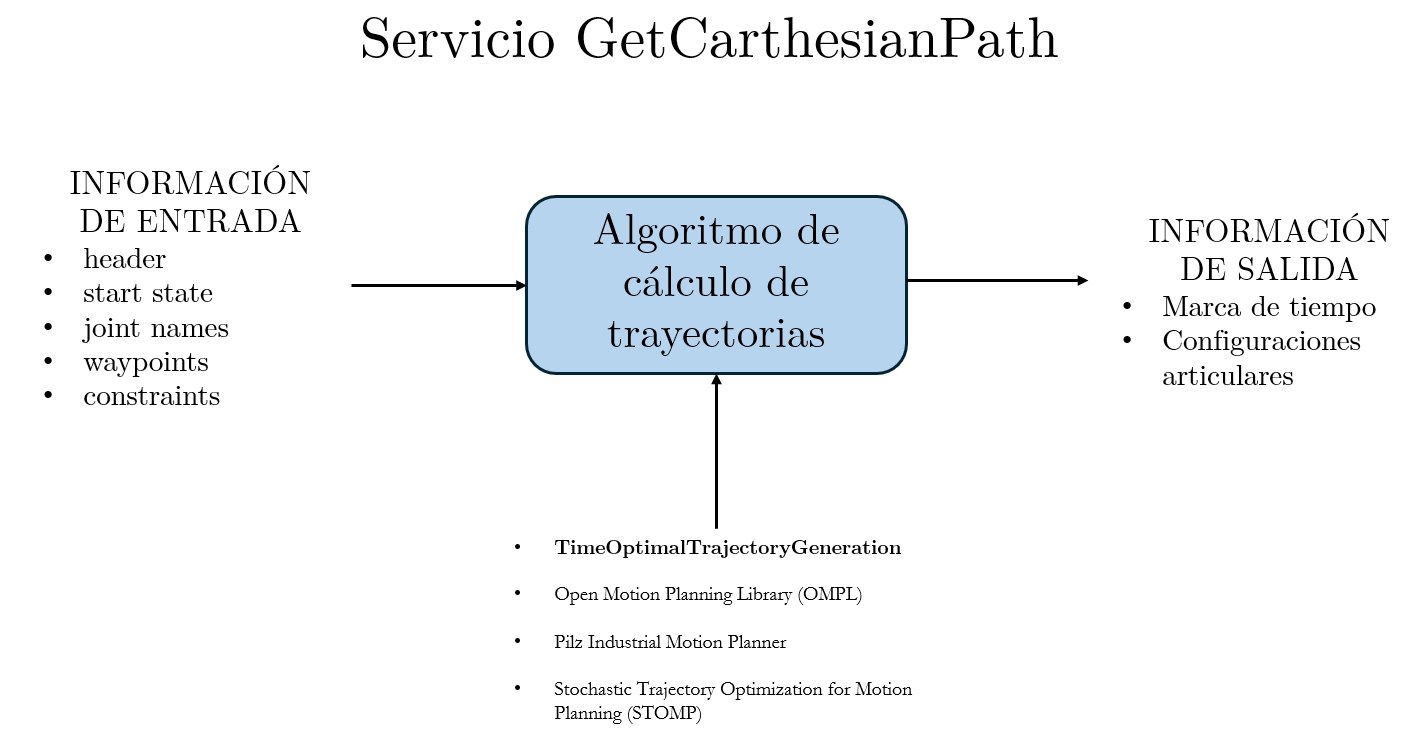
\includegraphics[scale=0.60]{figuras/esquema getcarthesianpath.png}
    \caption{Funcionamiento del servicio \textit{GetCarthesianPath}}
    \label{fig:esquema getcarthesianpath}
\end{figure}

Puesto que a priori no se tiene acceso al algoritmo de cálculo de trayectorias empleado durante la ejecución de dicha operación, el usuario debe definir cuál utilizar a través de parámetros externos. El algoritmo de cálculo de trayectorias o solver que se selecciona es el recomendado por la documentación oficial de MoveIt Humble, \textit{TimeOptimalTrajectoryGeneration} \cite{moveit_algoritmo_calculo_trayectoria}. El algoritmo (resaltado en negrita en la Figura \ref{fig:esquema getcarthesianpath} de entre otras alternativas) está enfocado en el cálculo de tiempos de ejecución óptimos para suavizar los movimientos calculados en base a las restricciones impuestas, por lo que se considera de utilidad para implementar un sistema de compensación automática de vibraciones e inercias del propio manipulador.

\subsubsection*{Ejecución de trayectorias}
\hypertarget{Ejecución de trayectorias}{}
\bookmark[level=subsubsection,dest=Ejecución de trayectorias]{Ejecución de trayectorias}

Una vez se ha descrito cómo se utiliza el algoritmo de cálculo implementado, se procede a desarrollar un nodo de ROS2 que utilice los servicios proporcionados por el controlador MoveIt para realizar el cálculo de la cinemática inversa y los movimientos necesarios a partir de la matriz de puntos resultado del proceso de \textit{slicing} de la pieza objetivo. Este nodo pertenece al paquete \textit{trayectories}, que se ha desarrollado con la intención se implementar un servicio especializado en dicha tarea.

El nodo responsable de esta operación tiene por nombre \textit{move\_l} y utilizando un enfoque \acrshort{POO} divide la ejecución de trayectorias en cuatro fases principales: lectura de matriz resultado de slicing, cálculo de trayectoria con MoveIt, definición de mensaje de acción ROS2 y ejecución de trayectoria. El funcionamiento del nodo se detalla en el algoritmo \ref{alg:algoritmo move l}. 

\begin{algorithm}[h!]
\caption{move\_l}\label{alg:algoritmo move l}
\begin{algorithmic}[1]
\Require Matriz de puntos de trayectoria de slicer en archivo CSV
\Ensure Instrucciones y ejecución automática de trayectoria robótica

\State Obtener el conjunto de puntos de la trayectoria de slicing.
\State Cargar los puntos del slicer en el vector \textit{waypoints}.

\State Invocar servicio \textit{GetCarthesianPath}.
\State Definir manipulador robótico y espacio de restricciones genéricas para \textit{GetCarthesianPath}.
\State Definir restricciones generales para la trayectoria deseada (si necesrio).
\State Cargar waypoints, modelo del manipulador y espacio de restricciones a la solicitud del servicio \textit{GetCarthesianPath}.
\State Cargar la solicitud a \textit{GetCarthesianPath}.

\While{No existe solución del servicio}
    \State Esperar.
\EndWhile

\If{Escala de velocidad $\neq$ 1}
    \State Ejecutar corrección de velocidad (algoritmo \ref{alg:algoritmo control proporcional velocidad})
\EndIf
\State Guardar trayectoria calculada en tabla CSV.

\State Invocar acción ROS2 de ejecución.
\State Asignar trayectoria calculada a la acción.
\State Ejecutar la acción.

\end{algorithmic}
\end{algorithm}

En este caso se opta por la ejecución del nodo siguiendo el modelo de arquitectura ROS2 acción cliente-servidor para habilitar al sistema de planificación offline del computador central de la autoridad suficiente para interrumpir la operación en cualquier momento, como si se tratase de un proceso asíncrono. 

La Figura \ref{fig:grafo move_l} muestra el grafo de nodos de ROS2 enfocado en \textit{move\_l}. En ella se aprecia que al emplearse un mecanismo de acción, se carga la información directamente a los mensajes de salida del entorno ROS2 (con el topic \textit{rosout}) y un mensaje que habilita la posibilidad de arrancar en paralelo el sistema de lectura de lectura de datos (con el topic \textit{arrancar\_logger\_topic}). Se debe tener en cuenta que por motivos de programación y creación de la interfaz ROS2 se define un nombre alternativo en la representación conocido como \textit{trayectory\_node\_cartesian}.

\begin{figure}[h!]
    \centering
    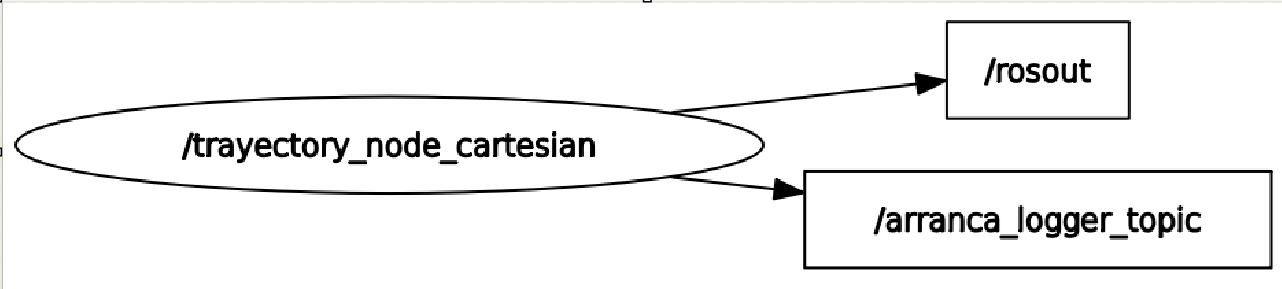
\includegraphics[scale=0.40]{figuras/grafo move_l.png}
    \caption{Grafo de conexionado de \textit{move\_l}}
    \label{fig:grafo move_l}
\end{figure}



\subsubsection*{Control de velocidad}
\hypertarget{Control de velocidad}{}
\bookmark[level=subsubsection,dest=Control de velocidad]{Control de velocidad}
\label{sec:control _velocidad}
Con el sistema de ejecución de trayectorias ya finalizado, queda implementar una acción de control que regule la velocidad de ejecución de la trayectoria calculada. El valor de esta acción es de vital importancia para regular otros aspectos como pueden ser la velocidad de deposición del material extruído o la seguridad del operario en el entorno real.

La primera aproximación que se realiza es establecer una velocidad límite como requisito de cálculo de trayectorias. Es decir se asigna un valor límite de velocidad articulación que se ha de respetar en todo momento modificando la definición del entorno virtual. Sin embargo, este enfoque muestra problemas de cálculo en trayectorias complejas realizadas en volúmenes pequeños como los que se desean alcanzar en este proyecto.

La siguiente aproximación pasa por definir una acción de control externa al cálculo de trayectorias efectuado gracias al solver integrado en MoveIt. Al tratarse de un sistema de fabricación aditiva, se supone que para favorecer la correcta deposición del material se realizarán movimientos a velocidad constante.

La variable de interés es la trayectoria resultado de la matriz de puntos proveniente del slicer, dicha trayectoria indicará los movimientos a efectuar y no se deben modificar. Sin embargo, la solución aportada por el algoritmo de cálculo debe incluir también unos valores para el instante de ejecución de cada movimiento, velocidad y aceleración. 

Aprovechando que el algoritmo \textit{TimeOptimalTrajectoryGeneration} aporta soluciones cinemáticas muy suavizadas, se opta por introducir una acción reguladora de tipo proporcional sobre los puntos que definen la trayectoria resultado. Es decir, definiendo de forma previa un factor de escala $K$ se puede decir que las nuevas velocidades, aceleraciones e instante de ejecución articulares serán respectivamente:

\begin{gather}
    \dot{q}= K\cdot \dot{q_o} \\
    \ddot{q}= K\cdot \ddot{q_o} \\
    t = t_o/K
\end{gather}

El algoritmo \ref{alg:algoritmo control proporcional velocidad} de implementación se incluye dentro del nodo cálculo y trazado de trayectoria \textit{move\_l}. Este algoritmo necesita de un factor de escala $K$ entre 0 y 1 como entrada, por lo que se introduce como un parámetro extra que por defecto queda definido con el valor de 1 para evitar ejecuciones innecesarias de la acción reguladora en caso de no querer modificar ninguna variable de ejecución.

\begin{algorithm}[h!]
\caption{Control proporcional de velocidad}\label{alg:algoritmo control proporcional velocidad}
\begin{algorithmic}[1]
\Require Factor de escala de velocidad $K$, trayectoria solución proporcionada por el servicio \textit{GetCarthesianPath}.
\Ensure Trayectoria solución con velocidad modificada según el factor de escala.

\State Obtener número de puntos de la trayectoria solución.
\State Definir un vector vacío de estados articulares modificados
\For{i $<$ Número puntos trayectoria}
    \State Multiplicar las i-velocidades articulares por el factor de escala.
    \State Multiplicar las i-aceleraciones articulares por el factor de escala.
    \State Dividir la i-marca de tiempo entre el factor de escala.
    \State Añadir la posición, velocidad y aceleración articulares modificadas del i-punto al final del vector de estados modificados.
    \State Añadir la marca de tiempo modificada del i-punto al final del vector de estados modificados.
\EndFor

\State Cargar el vector de trayectoria modificada como trayectoria solución.
\State Entregar como solución a ejecutar la trayectoria modificada.
\end{algorithmic}
\end{algorithm}

\section{Resultados y conclusiones}
En las siguientes secciones se evalúa el desempeño del sistema a través de tres ensayos que validarán su capacidad para evitar obstáculos, ejecutar las trayectorias deseadas para un sistema \acrshort{NPAM} y regular automáticamente la velocidad de movimiento del manipulador.

En base a dichos resultados y otras observaciones realizadas durante las etapas de desarrollo y validación, se comentarán una serie de ventajas y limitaciones presentes en el estado actual del sistema y las herramientas empleadas.

\subsection{Resultados}
Como sistema de evaluación del sistema, se realizaron varias pruebas según se avanzaba en cada una de las etapas de su desarrollo. La primera fue una prueba de colisiones controladas contra elementos reales que tenían su propia definición en el entorno virtual de aprendizaje offline. La segunda consistía en valorar la ejecución de trayectorias deseadas para un sistema robotizado \acrshort{NPAM} a la velocidad base establecida por el algoritmo de cálculo. La tercera era la responsable de validar la ejecución de esa misma trayectoria a diferentes velocidades utilizando el control proporcional de velocidad.

\subsubsection*{Colisiones con el entorno real}
\hypertarget{Colisiones con el entorno real}{}
\bookmark[level=subsubsection,dest=Colisiones con el entorno real]{Colisiones con el entorno real}

La validación de colisiones se realiza de forma controlada moviendo el manipulador robótico a bajas velocidades con ayuda del controlador Moveit y la interfaz gráfica de RViz. En este ensayo se propuso validar dos objetivos: (1) se respetan los límites virtuales definidos por los modelos \acrshort{CAD} introducidos en el entorno de aprendizaje offline pudiento interrumpir la orden de ejecución en caso de preveer una colisión y (2) se calculan automáticamente rutas alternativas por las que se pueda desplazar el \acrshort{TCP} al punto indicado.

Como elemento de pruebas se utilizó el soporte para albergar el sensor láser. La Figura \ref{fig: estado colisones entorno virtual} muestra el límite de colisión del modelo virtual del robot contra la esquina inferior del soporte, este desplazamiento fue definido con ayuda del controlador Moveit y su resultado de ejecución en el entorno real se aprecia en la Figura \ref{fig: validacion colision real}. 

La primera ejecución consistió en el desplazamiento del \acrshort{TCP} del manipulador al punto de colisión definido por el modelo virtual. Dicho punto se encuentra sobredimensionado respecto a la realidad para dejar un espacio mínimo de movimiento (aproximadamente 2 cm). 

\begin{figure}[h!]
    \centering
     \begin{subfigure}[h]{0.45\linewidth} 
        \centering
        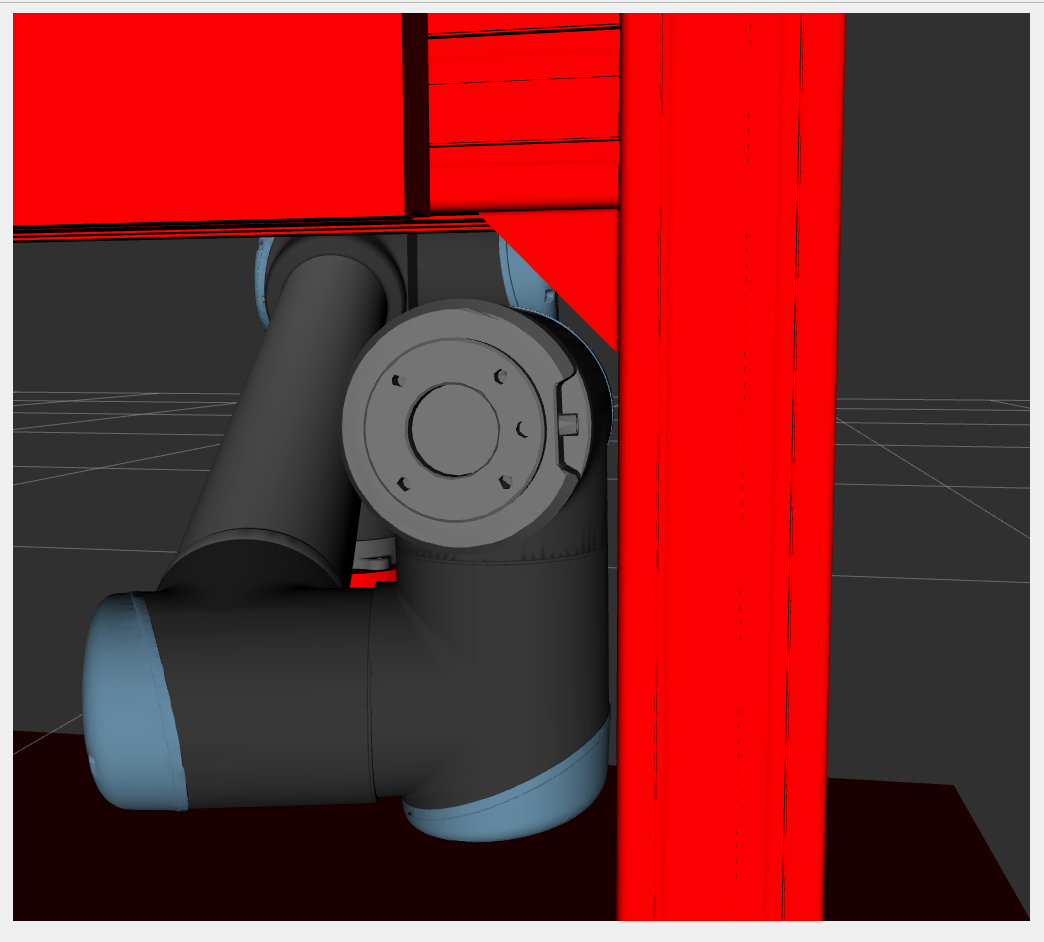
\includegraphics[scale=0.15]{figuras/estado colisiones entorno virtual.png}
        \caption{Colisión en el entorno virtual}
        \label{fig: estado colisones entorno virtual}
    \end{subfigure}
    \begin{subfigure}[h]{0.45\linewidth} 
        \centering
        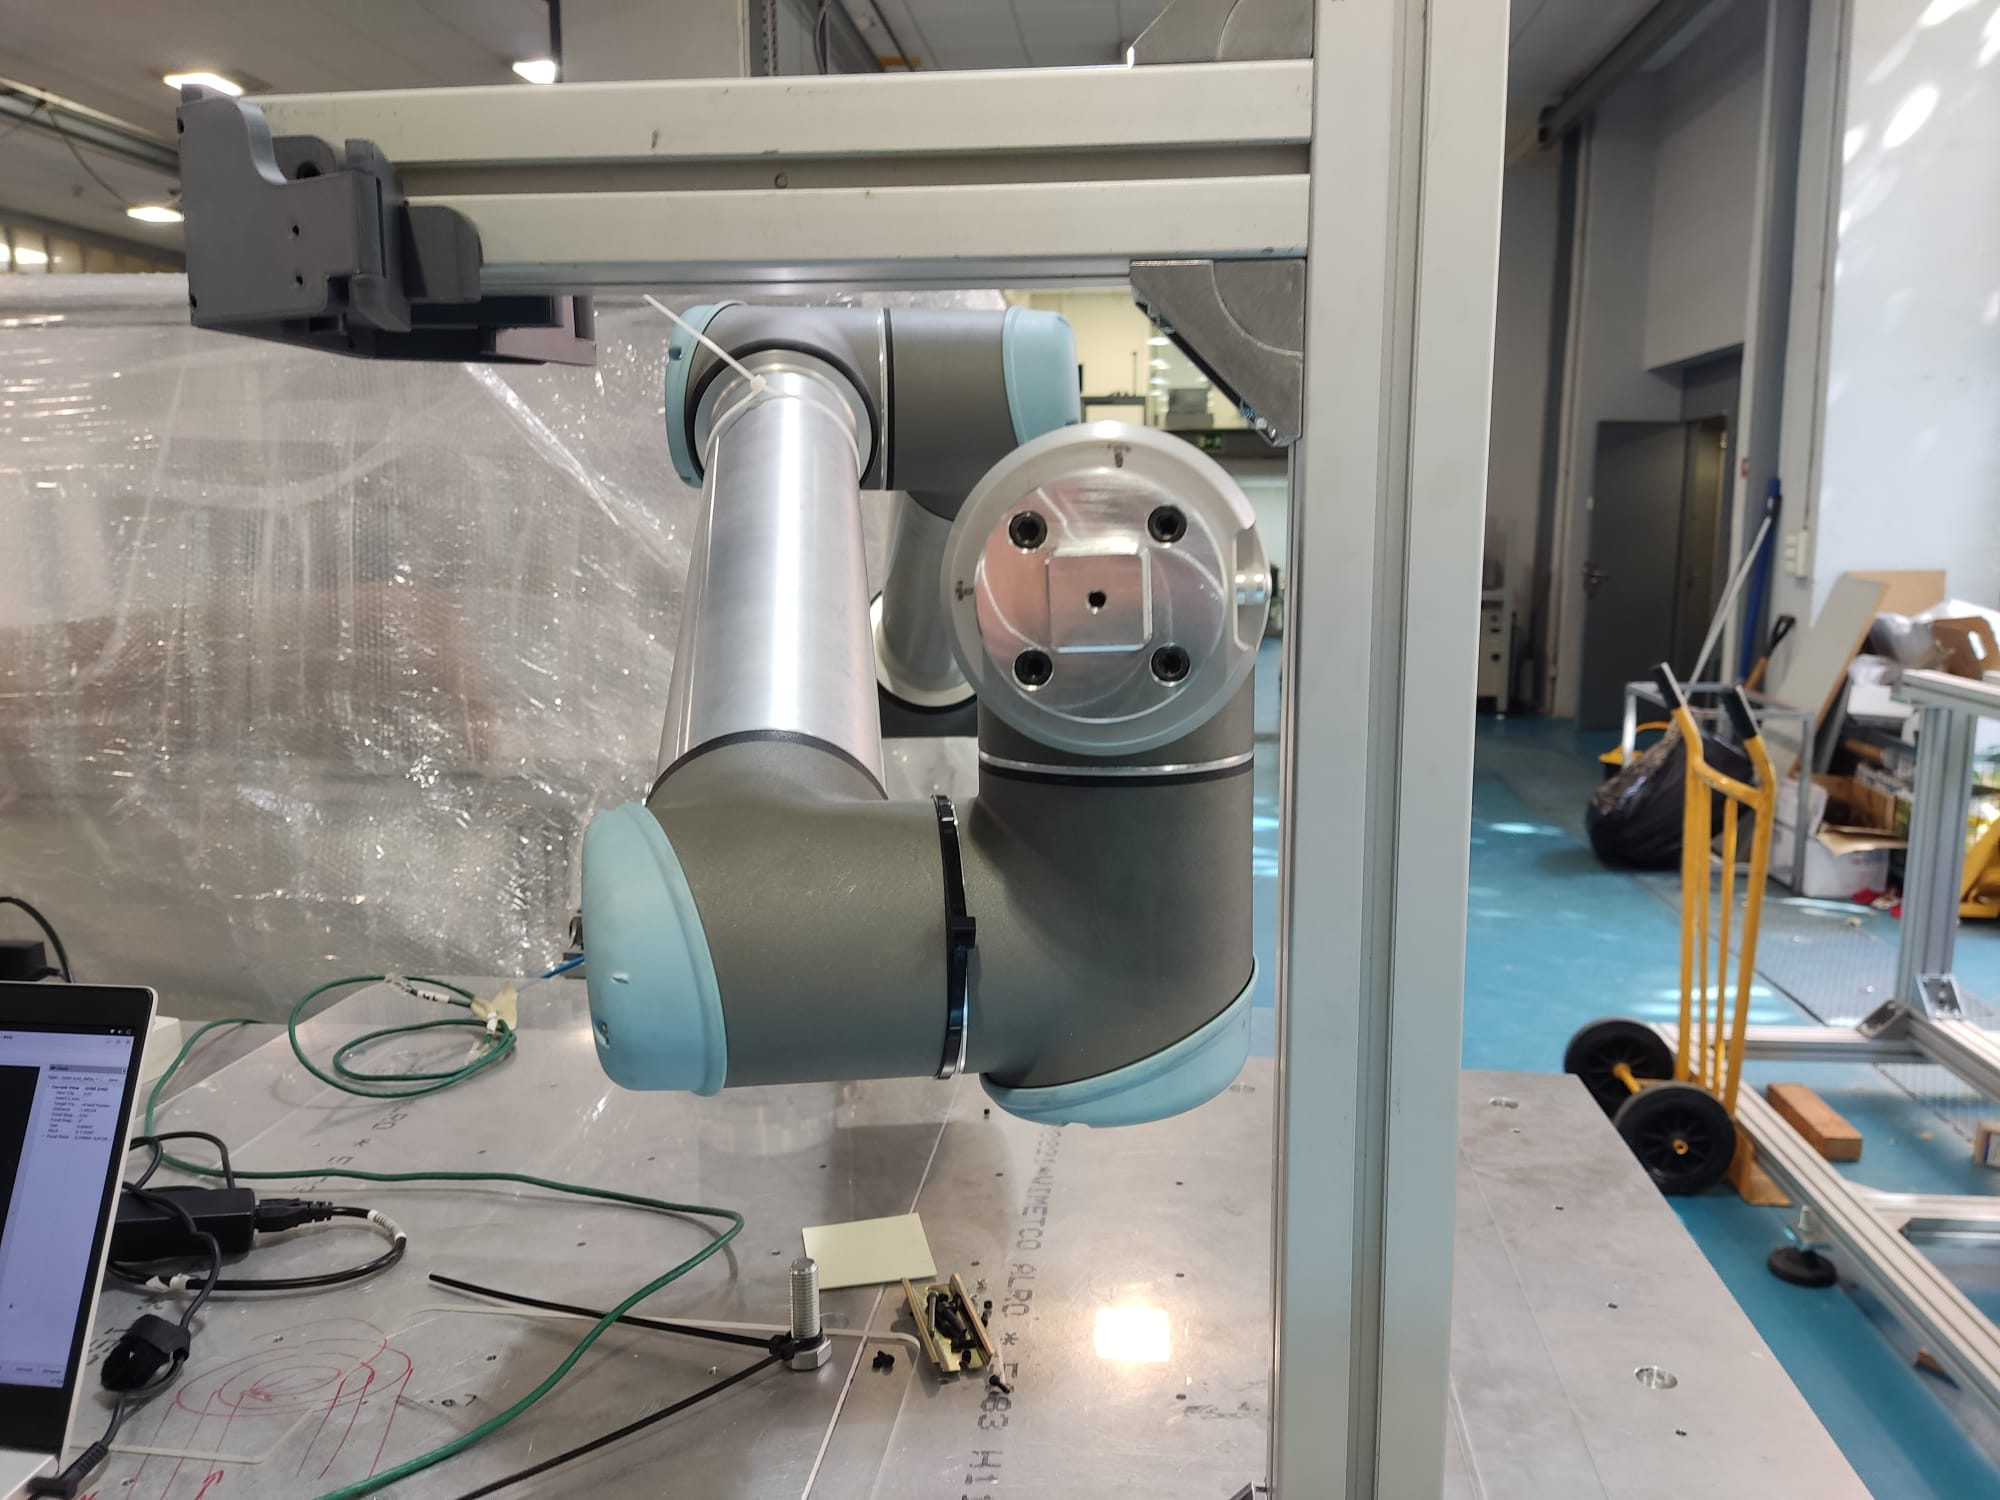
\includegraphics[scale=0.09]{figuras/validacion colision real.jpeg}
        \caption{Colisión en el entorno real}
        \label{fig: validacion colision real}
    \end{subfigure}
    \caption{Ensayo de colisiones}
    \label{fig: ensayo colisones percha}
\end{figure}

Tal como se aprecia en la Figura \ref{fig: ensayo colisones percha}, el resultado fue un éxito y para validar el objetivo número 2 se trató de desplazar el manipulador a muy baja velocidad contra la plataforma. El sistema de cálculo no permitió dicha ejecución y mostró un mensaje de error.

La validación del cálculo de rutas alternativas se realizó desplazando el manipulador desde su posición inicial a una justamente por encima del soporte. Es decir, el algoritmo de cálculo debía proponer una trayectoria alternativa que evitase el choque contra el soporte y otros elementos de la estación. 

En la Figura \ref{fig: ensayo colisiones rutas alternativas} se muestra la ejecución de dicho ensayo, el manipulador robótico se desplaza por sí mismo a una posición alejada del soporte para alcanzar la pose objetivo. Esta pose es visible en color naranja en la pantalla del computador central.

\begin{figure}[h!]
    \centering
    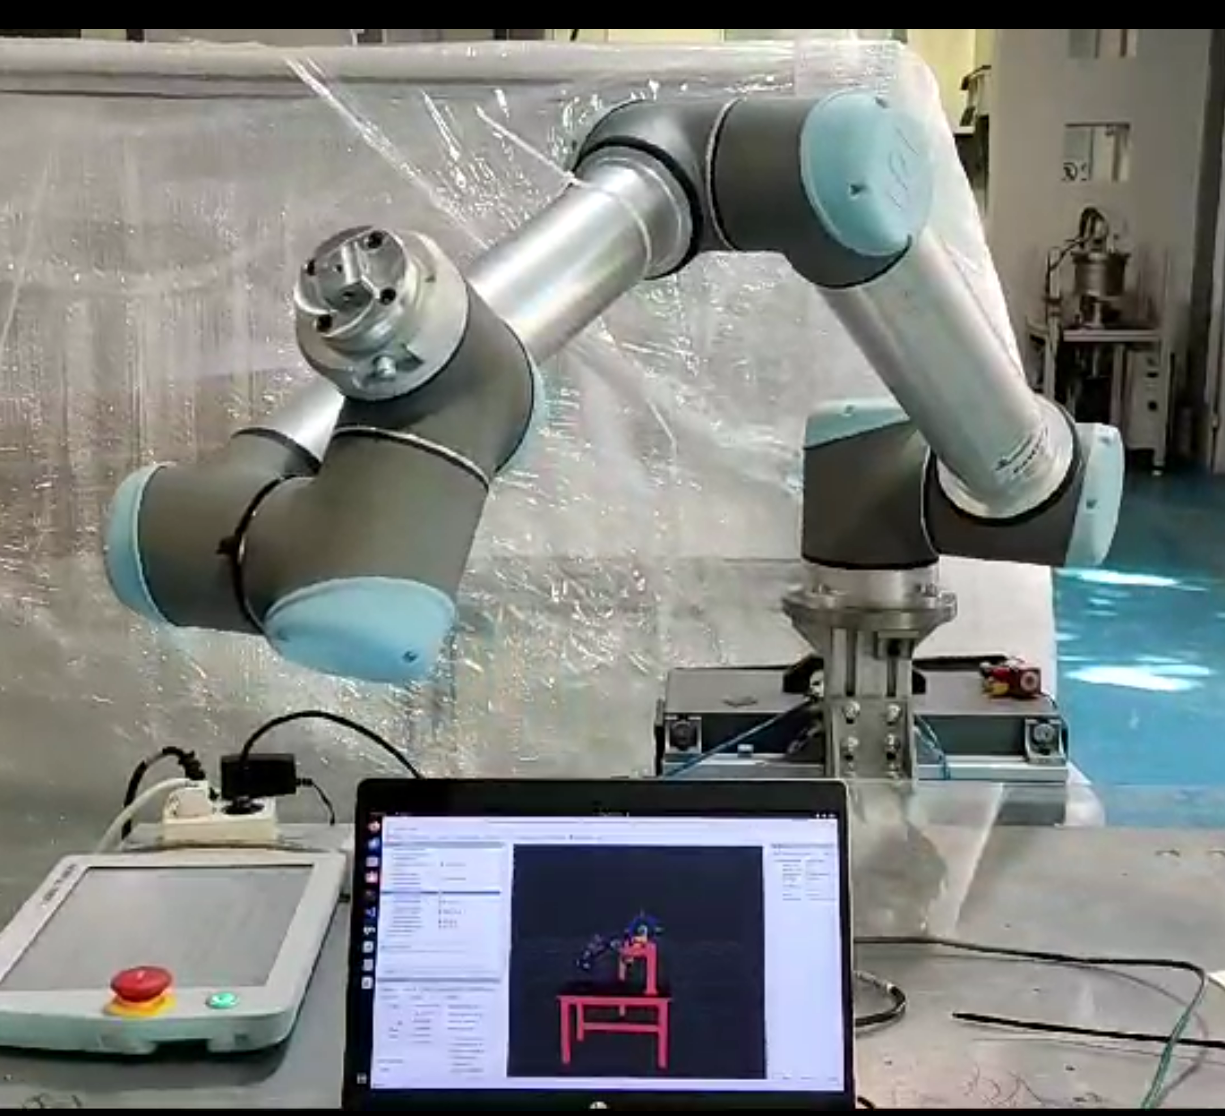
\includegraphics[scale=0.50]{figuras/ensayo colisiones rutas alternativas.png}
    \caption{Ensayo de colisiones. Rutas alternativas}
    \label{fig: ensayo colisiones rutas alternativas}
\end{figure}


\subsubsection*{Ejecución de trayectorias}
\hypertarget{Ejecución de trayectorias ensayo}{}
\bookmark[level=subsubsection,dest=Ejecución de trayectorias ensayo]{Ejecución de trayectorias}
\label{sec: resultados ejecución de trayectorias}

La ejecución de trayectorias \acrshort{NPAM} se valida tomando como referencia una pieza no planar que se desea realizar sobre la cama de impresión desarrollada por Iñaki Echepare \cite{TFM_IñakiEchepare}. En este caso, se utiliza el entorno virtualizado en su totalidad para validar la ejecución de la trayectoria objetivo. 

Esta trayectoria, presente en la Figura \ref{fig: validacion trayectoria objetivo}, representa la fabricación por capas de un semirresorte cilíndrico recto de 15 cm de longitud axial y 8 capas. La representación muestra la pieza deseada representada en diferentes capas no planares de con escala de color según altura de capa. Para una mejor compresión de los puntos, la imagen se representa con un sistema de referencia que asocia la cama de impresión con la brida del robot (o muñeca número 3 en su defecto).

\begin{figure}[h!]
    \centering
    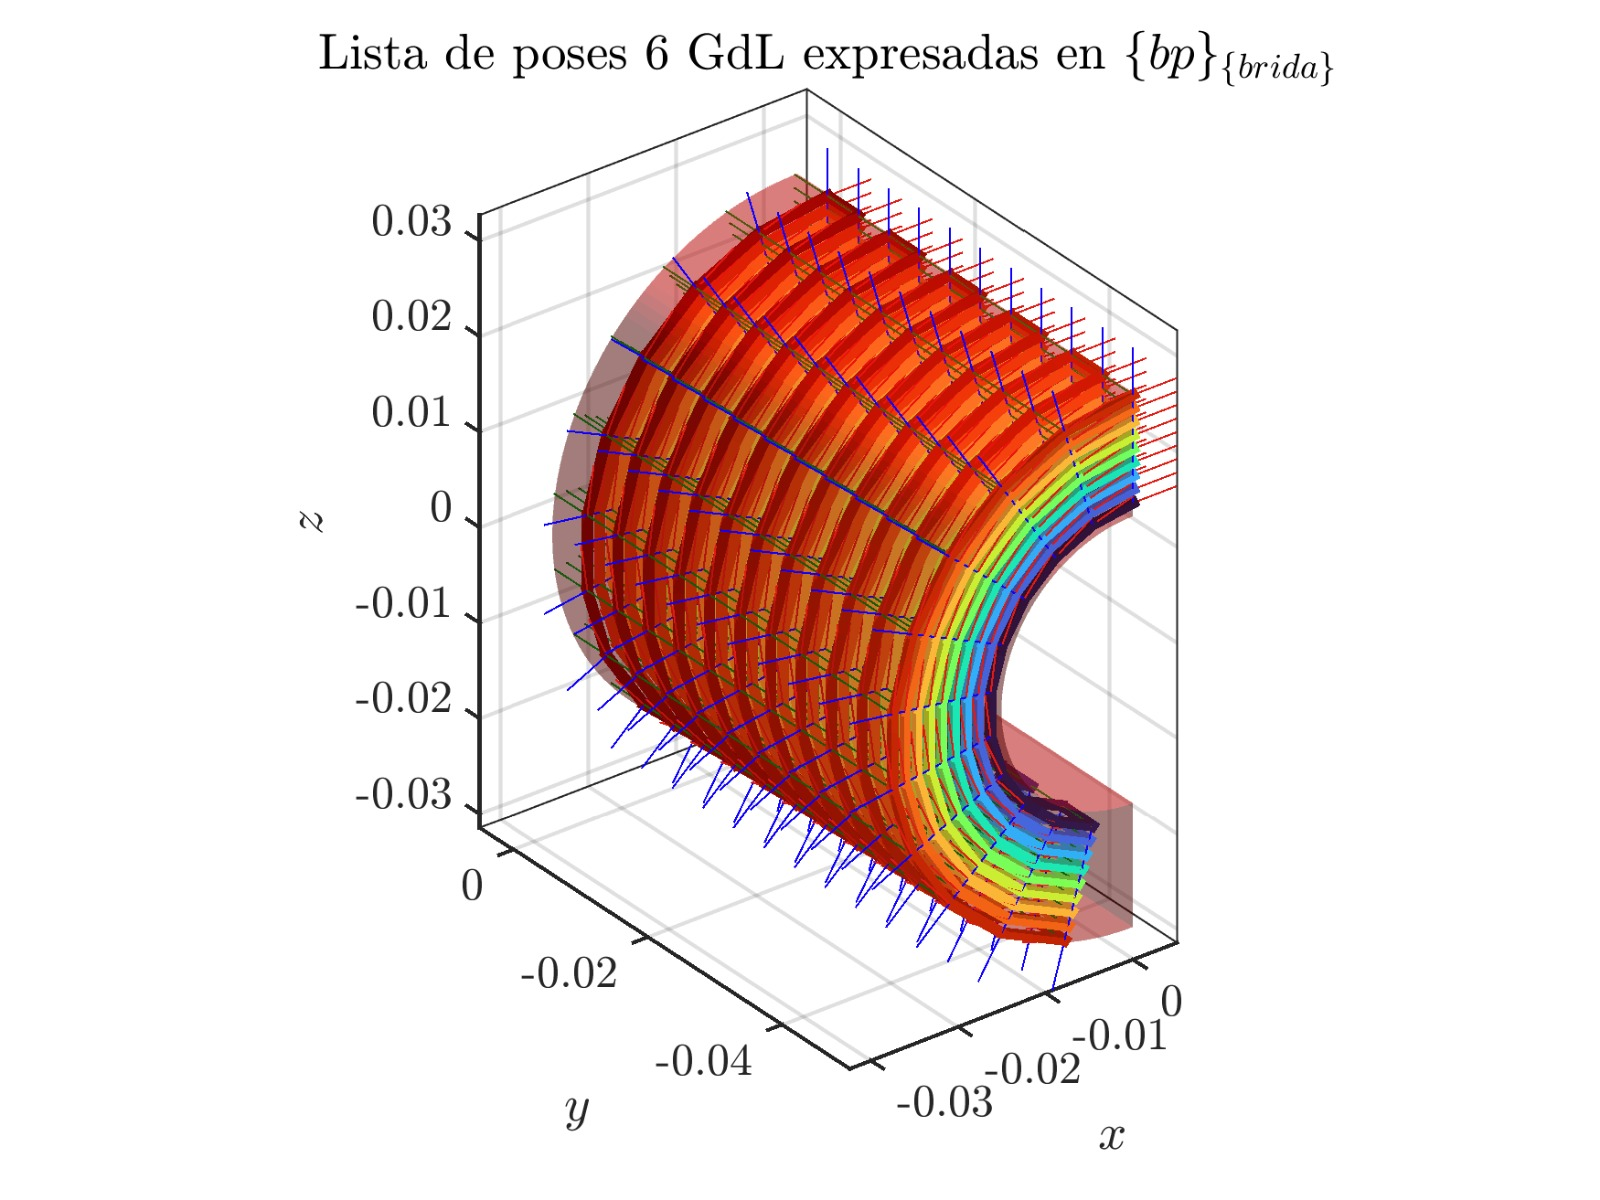
\includegraphics[scale=0.15]{figuras/validacion trayectoria npam trayectoria objetivo.jpg}
    \caption{Trayectoria \acrshort{NPAM} objetivo}
    \label{fig: validacion trayectoria objetivo}
\end{figure}

La Figura \ref{fig: validacion trayectoria npam ensayo realidad} muestra el proceso de ejecución de dicha trayectoria en el entorno real. Para validar que se mantiene una altura correspondiente al modelo definido por el slicer, se incorpora el sensor de distancia láser. Tanto los datos de configuraciones articulares como las medidas del sensor láser se registran en segundo plano con ayuda de los paquetes \textit{rutine\_launcher} y \textit{data\_logger} descritos respectivamente en los capítulos \ref{cap: diseno_arquitectura} y \ref{cap:lectura_datos}.

\begin{figure}[h!]
    \centering
    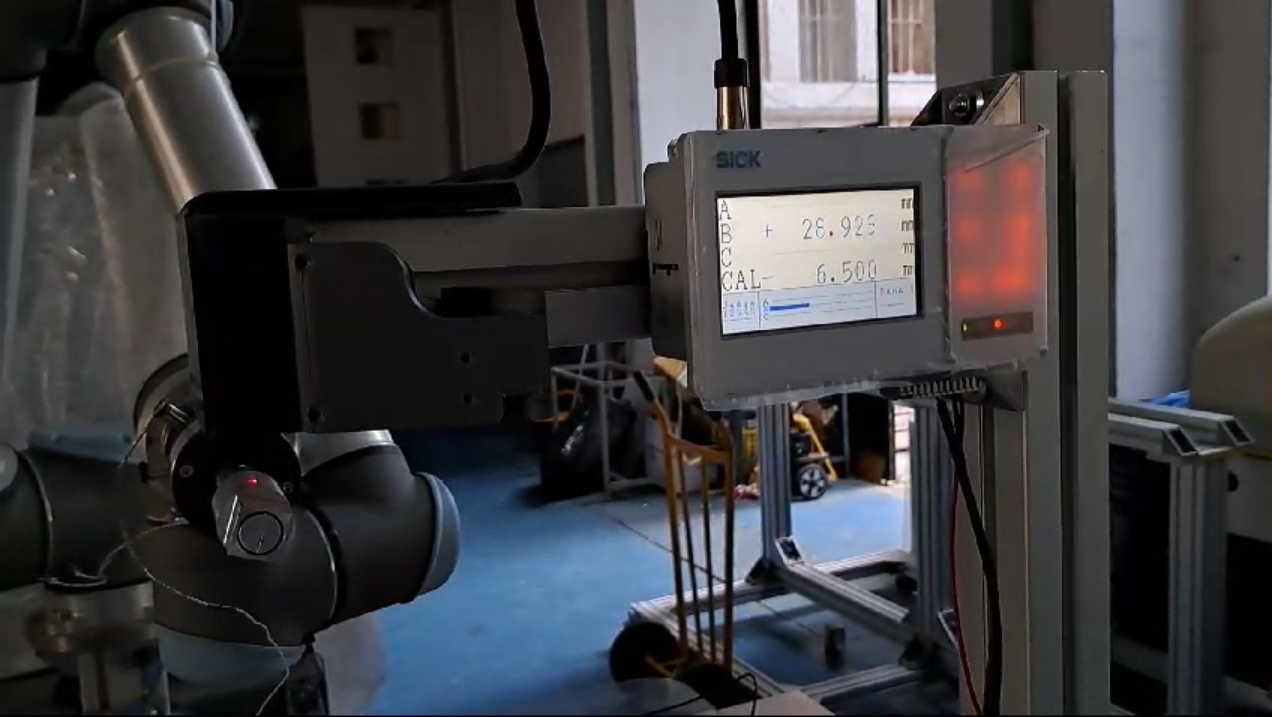
\includegraphics[scale=0.28]{figuras/validacion trayectoria npam ensayo realidad.png}
    \caption{Validación de ejecución de trayectoria \acrshort{NPAM}}
    \label{fig: validacion trayectoria npam ensayo realidad}
\end{figure}

A continuación se muestran los resultados de la trayectoria efectuada a un 10\% de la velocidad base proporcionada por el algoritmo de cálculo. Para una mejor interpretación de los resultados, únicamente se muestra la ejecución de las dos primeras capas de la pieza objetivo.

La Figura \ref{fig: posiciones ensayo trayectoria NPAM} muestra las posiciones articulares registradas por el manipulador robótico. De acuerdo con la forma de semirresorte deseada la articulación número 4 (correspondiente a la muñeca 3 \footnote{La numeración seguida por el controlador ROS2 y la establecida en el \acrshort{URDF} pueden diferir. La unidad empleada sigue el formato: q0\_hombro, q1\_codo, q2\_muñeca1, q3\_muñeca2, q4\_muñeca3, q5\_base. Queda a cargo del ingeniero responsable validar el orden empleado según su modelo de robot y unidad utilizada. \label{note: Aclaración número articulacionres ROS2}}.) es la que experimenta rotaciones continuadas a lo largo de los puntos ensayados. El resto de articulaciones son las responsables de compensar las inercias surgidas del movimiento, experimentando pequeñas variaciones que se deben a dicho ajuste.

\begin{figure}[h!]
    \centering
    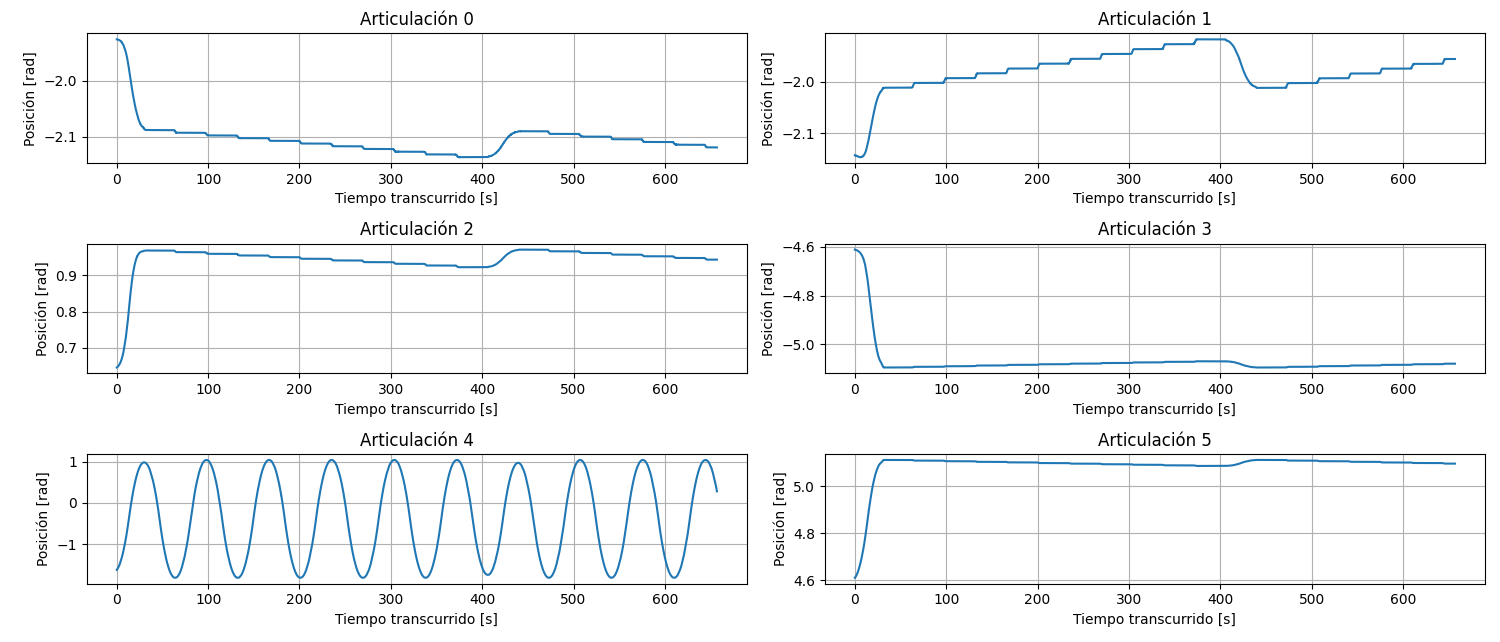
\includegraphics[scale=0.40]{figuras/ensayo_trayectorias/posicones escala 0.1.png}
    \caption{Ensayo de trayectoria \acrshort{NPAM}. Posiciones articulares}
    \label{fig: posiciones ensayo trayectoria NPAM}
\end{figure}

La Figura \ref{fig: velocidades ensayo trayectoria NPAM} muestra las velocidades registradas, en este caso se aprecia un movimiento prácticamente constante. Al efectuarse un movimiento a velocidades del orden de cm/s el valor en muchas ocasiones es cercano al nulo, y tan sólo destacan los picos de magnitud de orden 100 veces superior. La aparición de dichos picos se asocia con el ajuste automático que se ejerce durante el cálculo del movimiento para mantener un valor suavizado de la posición articular.

\begin{figure}[h!]
    \centering
    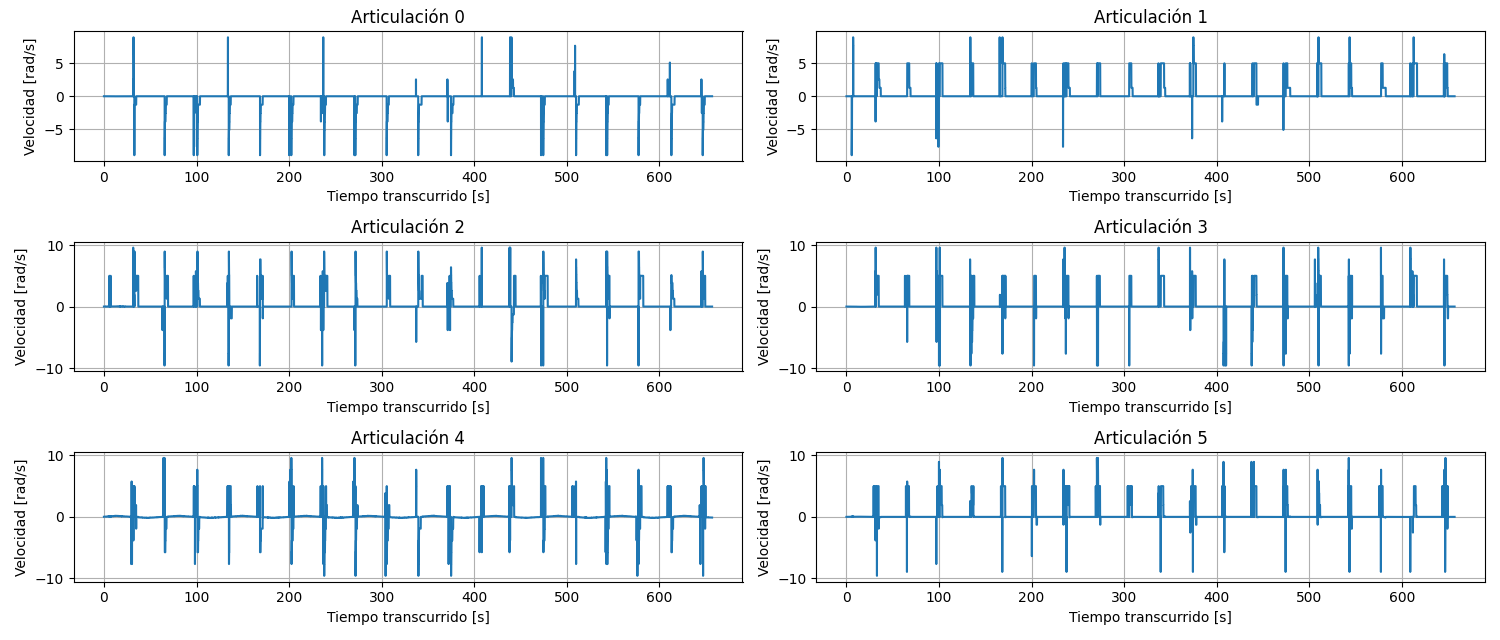
\includegraphics[scale=0.40]{figuras/ensayo_trayectorias/velocidad escala 0.1.png}
    \caption{Ensayo de trayectoria \acrshort{NPAM}. Velocidades articulares}
    \label{fig: velocidades ensayo trayectoria NPAM}
\end{figure}

En la Figura \ref{fig: esfuerzos ensayo trayectoria NPAM} se observa el comportamiento de los esfuerzos articulares registrados. Salvo por la articulación número 4 (correspondiente a la muñeca 3) se aprecia un registro promedio de tipo constante, con regiones de picos con un elevado ruido de fondo a causa de la compensación automática implementada por el controlador MoveIt. El caso más diferenciado es el de la articulación número 4, que se muestra en línea con las posiciones registradas un comportamiento claramente periódico. En el caso de la trayectoria ensayada, al tratarse de la articulación con mayor carga de trabajo es también la que experimenta mayor cantidad de compensaciones automáticas, motivo por la que también tiene un ruido de fondo promedio registrado de mayor amplitud.

\begin{figure}[H]
    \centering
    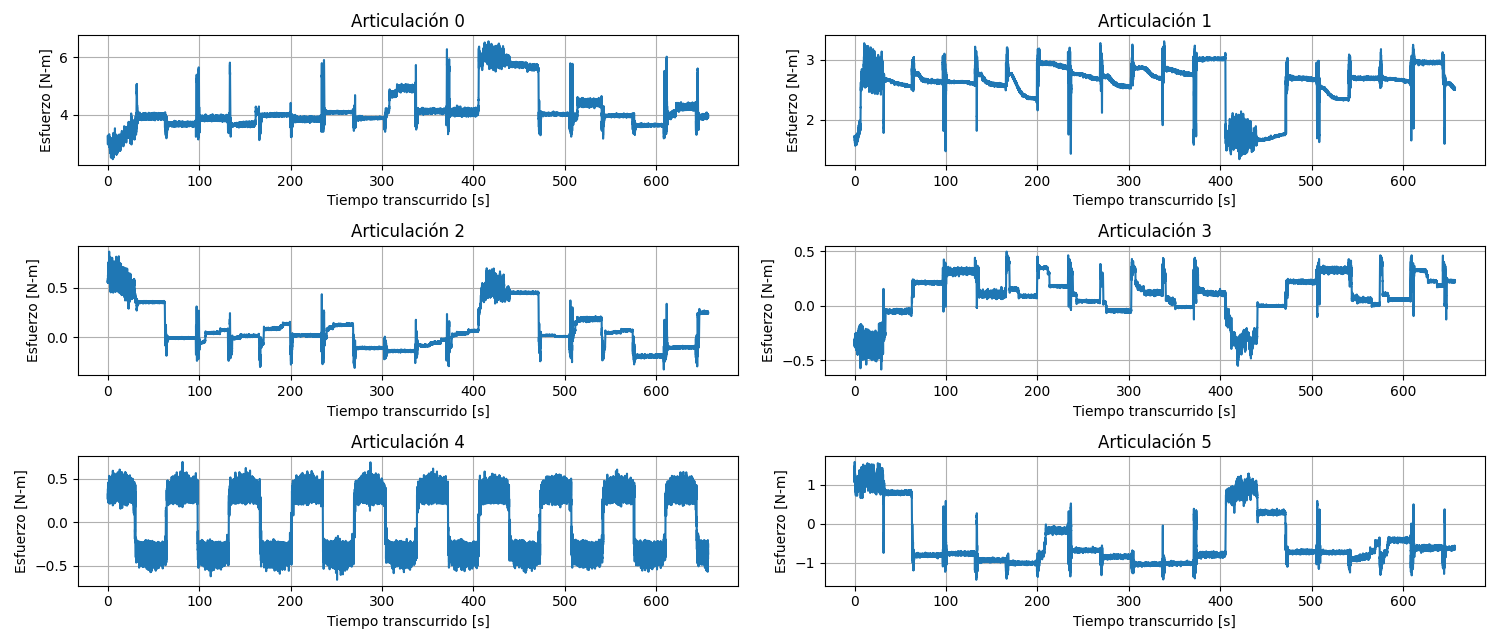
\includegraphics[scale=0.40]{figuras/ensayo_trayectorias/esfuerzos escala 0.1.png}
    \caption{Ensayo de trayectoria \acrshort{NPAM}. Esfuerzos articulares}
    \label{fig: esfuerzos ensayo trayectoria NPAM}
\end{figure}

Finalmente, la Figura \ref{fig: laser ensayo trayectoria NPAM} es la de mayor importancia en este ensayo. Es decir, es la responsable de mostrar que el modelo de cálculo se ajusta adecuadamente a la trayectoria objetivo comandada. Para ello se mide la distancia entre la cama móvil de impresión y el soporte que alojará el extrusor de material de la estación. El soporte también aloja el sensor láser de distancia que sirve como herramienta de validación. 

\begin{figure}[H]
    \centering
    \includegraphics[scale=0.70]{figuras/ensayo_trayectorias/laser escala 0.1 señalado.png}
    \caption{Ensayo de trayectoria \acrshort{NPAM}. Distancia al sensor láser}
    \label{fig: laser ensayo trayectoria NPAM}
\end{figure}

En este caso se asocia un comportamiento periódico con dos iteraciones diferenciadas, cada una correspondiente a una capa. Entre ambas iteraciones se señala con un círculo verde una variación abrupta de los valores registrados (en el caso de la Figura \ref{fig: laser ensayo trayectoria NPAM}, entre 320 y 400 segundos) que se corresponden con la finalización de una capa y el movimiento de la cama hasta el inicio de la siguiente. Los valores máximos de tipo sinusoidal están rodeados en rojo, en ellos se aprecia el cambio de altura al realizar cada semivuelta de la pieza objetivo. 

El comportamiento sinusoidal observado en cada capa sigue la línea trazada por referencias anteriores \cite{paper_Q1_Alvaro_Adrian}\cite{TFM_SanchoAmparo}, que indican que la presencia de cimas en forma de M está causada por los errores de calibración existentes entre el \acrshort{TCP} y el giro real. Estas diferencias encuentran su origen en un desalineamiento de los 6 \acrshort{DOF} al comandar movimientos de mayores revoluciones,  originando esta forma característica.

\subsubsection*{Control de velocidad}
\hypertarget{Control de velocidad ensayo}{}
\bookmark[level=subsubsection,dest=Control de velocidad ensayo]{Control de velocidad}
\label{sec: control velocidad ensayo}

En el ensayo de control de velocidad se registran los resultados obtenidos por el sensor de distancia láser para la misma trayectoria descrita en la Figura \ref{fig: validacion trayectoria objetivo}. En este caso, el parámetro variable es la velocidad de ejecución implementada según el factor de escala impuesto por la acción reguladora descrita en la sección anterior. 

Se realizan cuatro medidas de todo el trazado con factores de escala del 10\%, 20\%, 40\% y 60\% de la velocidad base propuesta por la solución original del controlador. Los resultados registrados se presentan en sus respectivas gráficas de posiciones articulares y distancia al láser (disponibles en el anexo \ref{cap: anexo control velocidad}).

Por parte del registro de configuraciones cinemáticas, se espera que un incremento progresivo de la velocidad de ejecución suponga un aumento de la frecuencia de las señales registradas y un incremento proporcional del tiempo de ejecución. En el caso del ensayo registrado, se debe tener en cuenta que la trayectoria comandada sólo incluye una parte de la cama de impresión, por lo que se espera que en los últimos segundos registrados se detecte un tramo de valor constante.

Un ejemplo del tipo de gráfico registrado es el de la Figura \ref{fig: control velocidad posiciones articulares 0.1}, en la que se muestra la trayectoria completa ejecutada al 10\% de la velocidad base. Nótese que en este tipo de gráficos las posiciones articulares registradas muestran pequeñas variaciones escalonadas que trazan una forma de diente de sierra. 

Este comportamiento es propio de los giros articulares efectuados por capa, donde se llega al límite determinado por la trayectoria objetivo y rápidamente se inicia la fabricación de la nueva capa. También se aprecian picos de los valores registrados, asociados a una compensación automática por parte del modelo de cálculo implementado por el controlador MoveIt.

\begin{figure}[h!]
    \centering
    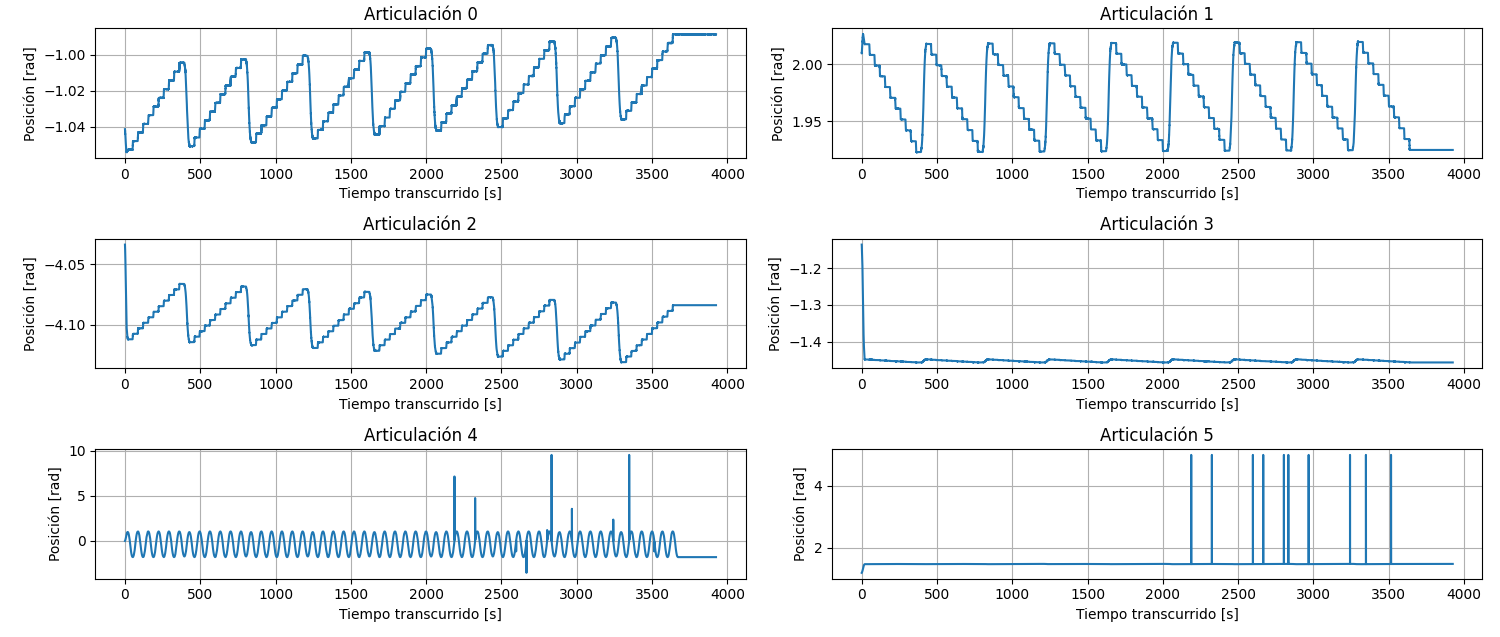
\includegraphics[scale=0.30]{figuras/ensayo_control_velocidad/posiciones articulares 0.1.png}
    \caption{Ensayo de control de velocidad. Factor de escala del 10\%. Posiciones articulares}
    \label{fig: control velocidad posiciones articulares 0.1}
\end{figure}

La Figura \ref{fig:ensayo control velocidad laser 0.1} representa la distancia a la cama de impresión medida con el sensor láser. Por motivos de ajuste de calibración del manipulador UR y del fondo de escala del sensor láser empleado (de unos 35 mm aproximadamente), no se pudo registrar la distancia correspondiente a  las 8 capas, por lo que solamente se dispone de 5. Esta gráfica se interpreta como la ejecución completa de los movimientos correspondientes a la Figura \ref{fig: laser ensayo trayectoria NPAM} en una nueva iteración. De forma análoga a dicha figura se aprecia el aumento de la distancia medida con cada nuevo cambio de capa. Los cambios de capa son fácilmente identificables gracias a los picos de distancia que tienen asociados. 

Para valorar la distancia de deposición presente durante el ensayo  con más facilidad, se efectúa una media móvil -coloreada en rojo- sobre los puntos registrados por el ensayo. En este caso se realizó un muestreo a una frecuencia de 100 HZ con un total de 300.000 muestras y se eligió una media móvil de alisado simple cada 3000 muestras.

\begin{figure}[H]
    \centering
    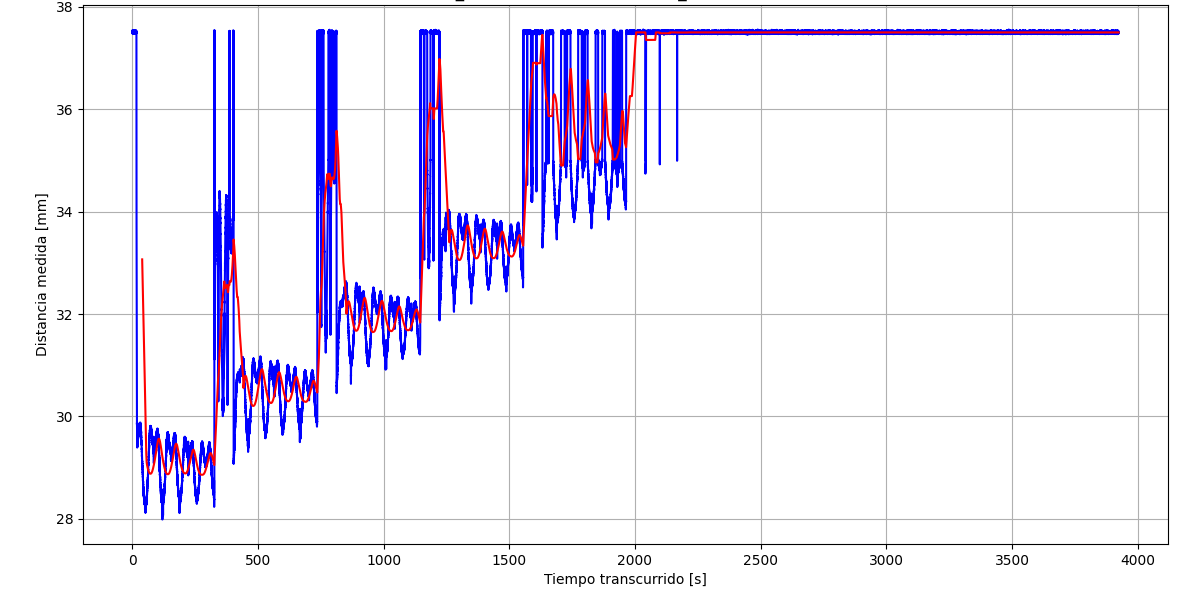
\includegraphics[scale=0.30]{figuras/ensayo_control_velocidad/laser 0.1.png}
    \caption{Ensayo de control de velocidad. Factor de escala del 10\%. Distancia al extrusor.}
    \label{fig:ensayo control velocidad laser 0.1}
\end{figure}

Los resultados de ejecución de los cuatro tiempos se muestran en la tabla \ref{tab: ensayo control velocidad tiempos}, donde se aprecia un incremento de tiempo correspondiente al valor base inversamente proporcional al factor de escala de la velocidad. Se señala con cursiva la solución base proporcionada por el algoritmo de cálculo, es decir, con un factor de escala del 100\%

% Please add the following required packages to your document preamble:
% \usepackage{graphicx}
\begin{table}[h!]
\centering
\resizebox{\columnwidth}{!}{%
\begin{tabular}{lcllllll}
\multicolumn{1}{c}{\textbf{Factor de escala {[}\%{]}}} &
  \multicolumn{1}{c}{\textbf{Tiempo de ejecución {[}min{]}}} &
  \multicolumn{1}{c}{\textbf{Velocidad de avance promedio {[}mm/s{]}}} &
  \multicolumn{1}{c}{\textbf{}} &
  \multicolumn{1}{c}{\textbf{}} &
  \multicolumn{1}{c}{\textbf{}} &
  \multicolumn{1}{c}{\textbf{}} &
  \multicolumn{1}{c}{\textbf{}} \\ \cline{1-3}
\multicolumn{1}{c}{\textit{100}} &
  \multicolumn{1}{c}{\textit{6,36}} &
  \multicolumn{1}{c}{\textit{3,15}} &
  \multicolumn{1}{r}{} &
   &
   &
   &
  \multicolumn{1}{c}{} \\
\multicolumn{1}{c}{10} &
  \multicolumn{1}{c}{66,65} &
  \multicolumn{1}{c}{0,30} &
  \multicolumn{1}{r}{} &
   &
   &
   &
  \multicolumn{1}{c}{} \\
\multicolumn{1}{c}{20} &
  \multicolumn{1}{c}{33,48} &
  \multicolumn{1}{c}{0,60} &
  \multicolumn{1}{r}{} &
   &
   &
   &
  \multicolumn{1}{c}{} \\
\multicolumn{1}{c}{40} &
  \multicolumn{1}{c}{15,78} &
  \multicolumn{1}{c}{1,27} &
  \textbf{} &
  \textbf{} &
  \textbf{} &
  \textbf{} &
  \multicolumn{1}{c}{} \\
\multicolumn{1}{c}{60} &
  \multicolumn{1}{c}{11,36} &
  \multicolumn{1}{c}{1,76} 
\end{tabular}%
}
\caption{Ensayo de control de velocidad. Tiempos registrados}
\label{tab: ensayo control velocidad tiempos}
\end{table}

Se calcula la velocidad de avance promedio de la pieza teniendo en cuenta la longitud axial y el tiempo de ejecución calculado automáticamente por el sistema, esto es, 15 cm de avance por 8 capas entre el tiempo total de ejecución. No se tienen en cuenta los intervalos de cambio de capa al efectuarse a velocidades lo suficientemente altas como para asignarse a intervalos de tiempo despreciables.

\subsection{Conclusiones}
En las siguientes líneas se presentan las principales ventajas y limitaciones del sistema desarrollado. Se seguirá el mismo orden utilizado en la sección de la metodología para finalizar con unas conclusiones generales del capítulo.

\subsubsection*{Entorno virtual}
\hypertarget{Entorno virtual}{}
\bookmark[level=subsubsection,dest=Entorno virtual]{Entorno virtual}

La construcción de un modelo virtual que sirva como referencia para un sistema de planificación offline ha demostrado ser una herramienta eficaz y de implementación sencilla. Por un lado la ejecución de movimientos sencillos con el manipulador, en los que el \acrshort{TCP} se desplaza únicamente de un punto a otro, ha resultado en una tarea sencilla y fácilmente controlable. Todo gracias a la integración prácticamente automática que se da entre las interfaces software proporcionadas por el controlador MoveIt, la interfaz gráfica RViz y el entorno de programación basado en ROS2. 

De igual modo, la implementación del controlador oficial para cobots UR en ROS2 ha permitido resolver de forma automática el problema de integrar una interfaz eficiente de accionamiento y comunicaciones entre los nodos representantes del robot real y el entorno virtualizado. Es decir, se ha podido asignar la responsabilidad sobre la tarea de control explícito de cada actuador interno del manipulador a un equipo software que, además, es fácilmente modificable para introducir los parámetros de calibración propios de la unidad. 

De este modo se consigue que el operario únicamente deba preocuparse de validar la correcta calibración entre el robot real y el modelo virtualizado. La clave para utilizar este tipo de procedimientos reside en dos puntos principales:
\begin{enumerate}
    \item La introducción de la calibración de la unidad introducida y los factores correctivos por parte del operario.
    \item La definición de objetos presentes en el entorno de trabajo real con los que el robot puede colisionar.
\end{enumerate}

Estos procesos ofrecen la integración de un sistema de restricciones de cálculo definidas en directo por el propio usuario en el entorno de trabajo real. Es decir, se abre la posibilidad de desarrollar un sistema de aprendizaje robótico de tipo híbrido en el que se combine la capacidad de cálculo de software con la acción correctora del ingeniero en planta.

\subsubsection*{Trazado de trayectorias}
\hypertarget{Trazado de trayectorias}{}
\bookmark[level=subsubsection,dest=Trazado de trayectorias]{Trazado de trayectorias}
Por parte del sistema de ejecución de trayectorias, se ha observado que la combinación de herramientas software aporta muy buenos resultados cuando se trata de la ejecución de trayectorias sencillas. Se define una trayectoria como \textit{sencilla} a aquel conjunto de posiciones adoptadas por el manipulador robótico que permiten desplazar su \acrshort{TCP} por el espacio real en un movimiento suavizado y en un volumen significativo. Es decir, un conjunto de puntos cartesianos en los que el controlador ROS2 puede realizar interpolaciones de tipo lineal con facilidad y con un tiempo de procesamiento reducido.

Las trayectorias de fabricación aditiva no planar suponen un conjunto elevado de puntos en el espacio que se han definido según una parametrización concreta \cite{TFM_SanchoAmparo}\cite{paper_Q1_Alvaro_Adrian} en la que se necesita realizar operaciones matemáticas complejas en un espacio reducido. Esto es, a priori no existe una garantía completa de que el sistema de lectura de la matriz de puntos ejecute la trayectoria proveniente del slicer sin poner en riesgo la integridad del entorno de trabajo.

Este problema se asocia con que la planificación seguida por el slicer no planar empleado difiere en el ajuste de los parámetros de cálculo de la cinemática inversa que emplea el modelo utilizado por el controlador MoveIt, en este caso \textit{TimeOptimalTrajectoryGeneration}. Es decir, el uso de un sistema de cálculo de cinemática inversa ya optimizado para ROS2 supone al mismo tiempo la mayor ventaja e inconveniente del sistema desarrollado.

Por un lado se tiene un procedimiento automático enfocado en la optimización de tiempo entre los puntos calculados, es decir, en la ejecución de a priori cualquier trayectoria a altas velocidades y con un movimiento suavizado que no depende en ningún momento del error de cálculo humano. Por otro lado, se debe tener especial cuidado con el algoritmo de cálculo de trayectorias seleccionado en el momento de implementación, ya que la solución proveniente del slicer puede diferir en el ajuste de ciertos parámetros que fuercen al manipulador a adoptar poses innecesariamente complicadas para la tarea efectuada.

Un ejemplo de dicha problemática se describe con ayuda de la Figura \ref{fig: problematica ejecucion trayectoria}. En este caso, se procedió directamente a efectuar la trayectoria no planar definida por la Figura \ref{fig: validacion trayectoria objetivo} sin realizar un ajuste previo de los parámetros de cálculo en el slicer \acrshort{NPAM} para coincidir con el solver del sistema ROS2.

\begin{figure}[H]
    \centering
    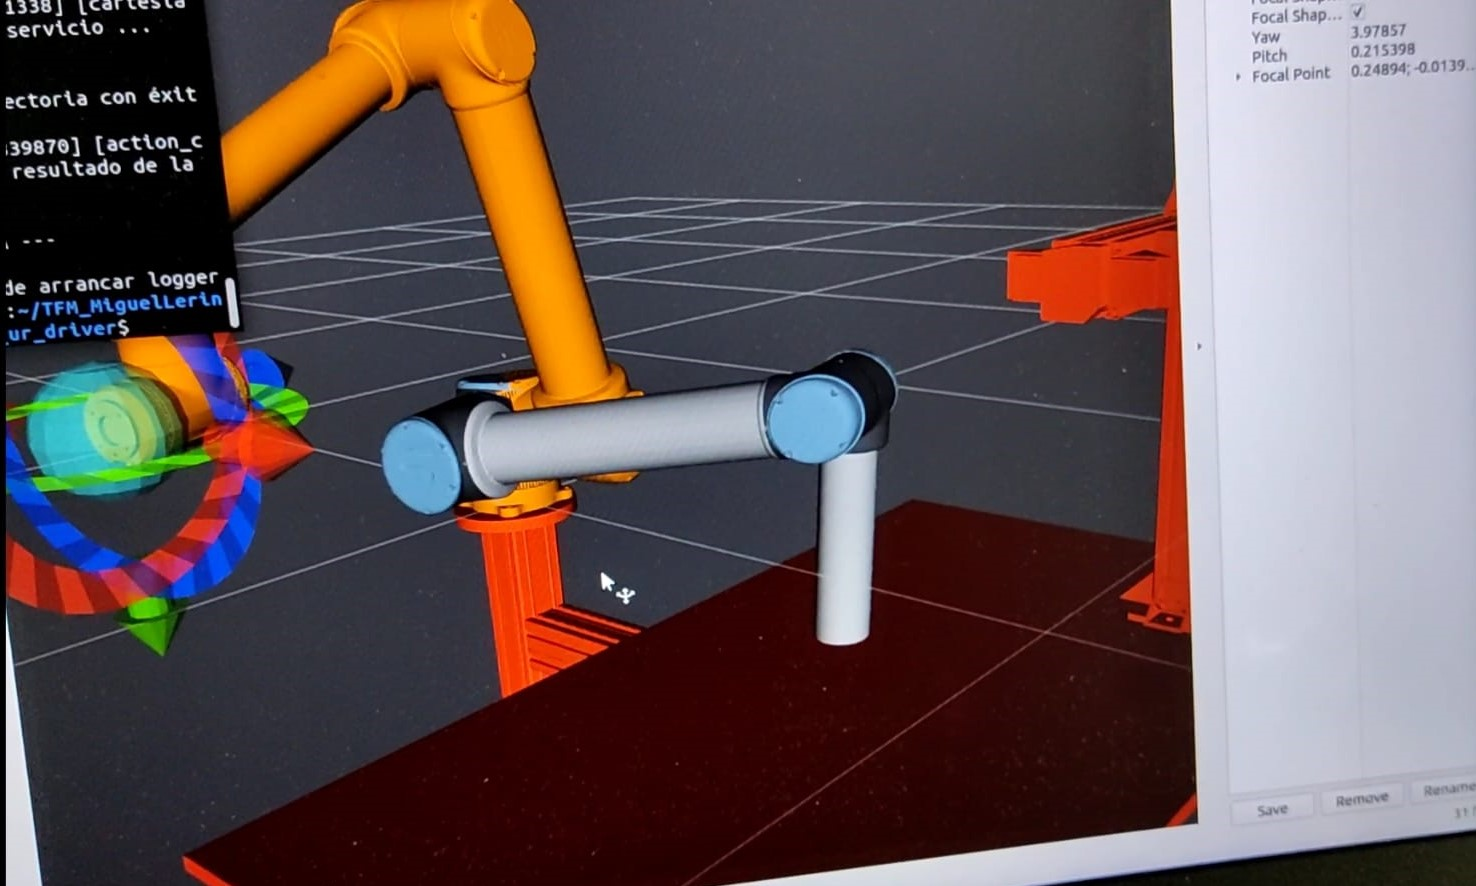
\includegraphics[scale=0.25]{figuras/problematica ejecucion trayectoria.jpeg}
    \caption{Trayectoria de colisión que no respeta las restricciones impuestas}
    \label{fig: problematica ejecucion trayectoria}
\end{figure}

El resultado de dicha problemática es la adopción de poses que ponen en riesgo a todo el entorno de trabajo de la estación robotizada, como se aprecia en la Figura \ref{fig: problematica ejecucion trayectoria}, donde el modelo simulado omite las restricciones de los modelos \acrshort{CAD} integrados y los atraviesa. Este comportamiento es el resultado de un cálculo incorrecto que puede suponer un riesgo elevado en caso de comandar su ejecución al cobot real, punto donde el operario ya no posee ningún poder adicional a la interrupción de emergencia del proceso.

La solución aportada para a esta problemática pasa por realizar un estudio previo de las diferencias en el procedimiento de cálculo implementado por el solver de slicing \acrshort{NPAM} y el de la cinemática inversa con el robot. Resultados mostrados en la sección \ref{sec: resultados ejecución de trayectorias}, que abren la puerta a futuros proyectos que se pueden enfocar en:

\begin{itemize}
    \item Desarrollar de un procedimiento de cálculo común a ambas etapas del flujo de trabajo.
    \item Implementar un sistema de detección previa de errores antes de mandar ejecutar dicha trayectoria. Es decir que se notifique el riesgo de colisión independientemente del uso del entorno simulado o real.
    \item Validar alinealidades y diferencias en los modelos de cálculo de trayectorias no planares y cinemáticas utilizadas.
    \item Investigar y/o evaluar de otros modelos de cálculo y ejecución de trayectorias complejas, especialmente no planares dada la naturaleza del trabajo.
\end{itemize}


\subsubsection*{Control de velocidad}
\hypertarget{Control de velocidad conclusiones}{}
\bookmark[level=subsubsection,dest=Control de velocidad conclusiones]{Control de velocidad}
\label{sec: control velocidad conclusiones}

La acción de control de velocidad implementada ha mostrado resultados positivos en cuanto a la reducción de la velocidad de ejecución sin modificar el resultado del cálculo de trayectoria. Lo que favorece el uso de validaciones en el entorno de trabajo real que ayuden a mejorar la ejecución del proceso de fabricación y la calibración del manipulador.

El principal inconveniente del método de regulación implementado reside en su dependencia de una solución previa existente. Es decir, al efectuar una acción correctora de velocidad, aceleración y tiempo de ejecución posterior a la etapa de cálculo de trayectorias la única forma de integrarla es en el interior de un procedimiento de mayor grado de abstracción, como se realiza en el algoritmo \ref{alg:algoritmo move l}.

De igual modo, otra limitación presente en el estado actual del controlador MoveIt utilizado es la ausencia de un conjunto de mensajes que impongan restricciones sobre la trayectoria resultado en forma de movimientos de avance del \acrshort{TCP} de acuerdo con una representación cartesiana. Precisamente por ello, algunas mejoras propuestas de cara a futuros proyectos pueden pasar por:
\begin{itemize}
    \item Implementar una acción reguladora no dependiente de la solución proporcionada por el controlador.
    \item Desarrollar un sistema de transformación entre la velocidad del \acrshort{TCP} deseada y los correspondientes valores articulares.
    \item Evaluar el comportamiento de la acción reguladora con otros algoritmos de cálculo de trayectorias y proponer otros modelos de regulación automática como puede ser la inserción de un regulador tipo PID.
\end{itemize}


\subsubsection*{Conclusiones del capítulo}
\hypertarget{Conclusiones del capítulo}{}
\bookmark[level=subsubsection,dest=Conclusiones del capítulo]{Conclusiones del capítulo}
\label{sec: conclusiones capítulo trayectorias} 

El sistema desarrollado ha demostrado ser útil para el cálculo y ejecución de trayectorias basado en un modelo de aprendizaje offline con capacidad para integrar parámetros provenientes de un aprendizaje offline, abriendo la puerta a un futuro trabajo con un sistema de aprendizaje híbrido.

Se ha validado con éxito que un entorno de programación software basado en ROS2 es capaz de procesar y ejecutar automáticamente trayectorias de fabricación aditiva robotizada, de tipo no planar en este caso. No obstante se debe tener en cuenta ciertas limitaciones asociadas al estado actual de las herramientas empleadas como son las diferencias existentes entre el algoritmo de cálculo de cinemática inversa disponible y el algoritmo de slicing, la existencia de desviaciones en la calibración introducida en el modelo virtual o la necesidad de introducir una acción de control posterior al proceso de cálculo.

Es decir, pese a que se ha demostrado que es posible la ejecución automática de trayectorias complejas de impresión basadas en un modelo de programación ROS2 todavía se pueden introducir nuevas mejoras enfocadas a que no sea estrictamente necesario que el operario deje toda la responsabilidad al sistema en la planificación y regulación de trayectorias de impresión.